\documentclass{article}

% if you need to pass options to natbib, use, e.g.:
%     \PassOptionsToPackage{numbers, compress}{natbib}
% before loading neurips_2021

% ready for submission
\usepackage{neurips_2021}

% to compile a preprint version, e.g., for submission to arXiv, add add the
% [preprint] option:
%     \usepackage[preprint]{neurips_2021}

% to compile a camera-ready version, add the [final] option, e.g.:
%     \usepackage[final]{neurips_2021}

% to avoid loading the natbib package, add option nonatbib:
%    \usepackage[nonatbib]{neurips_2021}

\usepackage[utf8]{inputenc} % allow utf-8 input
\usepackage[T1]{fontenc}    % use 8-bit T1 fonts
%\usepackage{hyperref}       % hyperlinks
\usepackage{url}            % simple URL typesetting
\usepackage{booktabs}       % professional-quality tables
\usepackage{amsfonts}       % blackboard math symbols
\usepackage{nicefrac}       % compact symbols for 1/2, etc.
\usepackage{microtype}      % microtypography
\usepackage{xcolor}         % colors

\usepackage{microtype}
\usepackage{graphicx}
\usepackage{subfigure}
\usepackage{booktabs} % for professional tables

\usepackage{amssymb}
\usepackage{amsfonts}     
\usepackage{epsfig}
\usepackage{algorithm}
\usepackage{algorithmic}
\usepackage{wrapfig}
\usepackage{amsthm}
\usepackage{balance}
\usepackage{mathtools} 
\usepackage{extarrows} 
\usepackage{microtype}
\usepackage{url}
\usepackage{xcolor}
\usepackage{subfigure}
\usepackage[font=small,labelfont=bf]{caption}

\definecolor{ao(english)}{rgb}{0.0, 0.5, 0.0}
\definecolor{lavander}{cmyk}{0,0.48,0,0}
\definecolor{violet}{cmyk}{0.79,0.88,0,0}
\definecolor{burntorange}{cmyk}{0,0.52,1,0}
\usepackage[colorlinks=true,linkcolor=ao(english),urlcolor=blue,citecolor=burntorange]{hyperref}
\usepackage{multirow}

\newcommand{\zz}[1]{\textcolor{blue}{#1}}
\newcommand{\Xc}{{\mathcal X}}
\newcommand{\Zc}{{\mathcal Z}}
\newcommand{\Pn}{\mathbb P^{(n)}}
\newcommand{\Qn}{\mathbb Q^{(n)}}
\newcommand{\pr}{{\mathbb P}}
\newcommand{\ex}{\mathbb E}
\newtheorem{lemma}{Lemma}
\newtheorem{remark}{Remark}
\newtheorem{definition}{Definition}
\newtheorem{theorem}{Theorem}
\newcommand{\RN}[1]{%
	\textup{\lowercase\expandafter{\it \romannumeral#1}}%
}
%%%%% NEW MATH DEFINITIONS %%%%%

\usepackage{amsmath,amsfonts,bm}

% Mark sections of captions for referring to divisions of figures
\newcommand{\figleft}{{\em (Left)}}
\newcommand{\figcenter}{{\em (Center)}}
\newcommand{\figright}{{\em (Right)}}
\newcommand{\figtop}{{\em (Top)}}
\newcommand{\figbottom}{{\em (Bottom)}}
\newcommand{\captiona}{{\em (a)}}
\newcommand{\captionb}{{\em (b)}}
\newcommand{\captionc}{{\em (c)}}
\newcommand{\captiond}{{\em (d)}}

% Highlight a newly defined term
\newcommand{\newterm}[1]{{\bf #1}}


% Figure reference, lower-case.
\def\figref#1{figure~\ref{#1}}
% Figure reference, capital. For start of sentence
\def\Figref#1{Figure~\ref{#1}}
\def\twofigref#1#2{figures \ref{#1} and \ref{#2}}
\def\quadfigref#1#2#3#4{figures \ref{#1}, \ref{#2}, \ref{#3} and \ref{#4}}
% Section reference, lower-case.
\def\secref#1{section~\ref{#1}}
% Section reference, capital.
\def\Secref#1{Section~\ref{#1}}
% Reference to two sections.
\def\twosecrefs#1#2{sections \ref{#1} and \ref{#2}}
% Reference to three sections.
\def\secrefs#1#2#3{sections \ref{#1}, \ref{#2} and \ref{#3}}
% Reference to an equation, lower-case.
\def\eqref#1{equation~\ref{#1}}
% Reference to an equation, upper case
\def\Eqref#1{Equation~\ref{#1}}
% A raw reference to an equation---avoid using if possible
\def\plaineqref#1{\ref{#1}}
% Reference to a chapter, lower-case.
\def\chapref#1{chapter~\ref{#1}}
% Reference to an equation, upper case.
\def\Chapref#1{Chapter~\ref{#1}}
% Reference to a range of chapters
\def\rangechapref#1#2{chapters\ref{#1}--\ref{#2}}
% Reference to an algorithm, lower-case.
\def\algref#1{algorithm~\ref{#1}}
% Reference to an algorithm, upper case.
\def\Algref#1{Algorithm~\ref{#1}}
\def\twoalgref#1#2{algorithms \ref{#1} and \ref{#2}}
\def\Twoalgref#1#2{Algorithms \ref{#1} and \ref{#2}}
% Reference to a part, lower case
\def\partref#1{part~\ref{#1}}
% Reference to a part, upper case
\def\Partref#1{Part~\ref{#1}}
\def\twopartref#1#2{parts \ref{#1} and \ref{#2}}

\def\ceil#1{\lceil #1 \rceil}
\def\floor#1{\lfloor #1 \rfloor}
\def\1{\bm{1}}
\newcommand{\train}{\mathcal{D}}
\newcommand{\valid}{\mathcal{D_{\mathrm{valid}}}}
\newcommand{\test}{\mathcal{D_{\mathrm{test}}}}

\def\eps{{\epsilon}}


% Random variables
\def\reta{{\textnormal{$\eta$}}}
\def\ra{{\textnormal{a}}}
\def\rb{{\textnormal{b}}}
\def\rc{{\textnormal{c}}}
\def\rd{{\textnormal{d}}}
\def\re{{\textnormal{e}}}
\def\rf{{\textnormal{f}}}
\def\rg{{\textnormal{g}}}
\def\rh{{\textnormal{h}}}
\def\ri{{\textnormal{i}}}
\def\rj{{\textnormal{j}}}
\def\rk{{\textnormal{k}}}
\def\rl{{\textnormal{l}}}
% rm is already a command, just don't name any random variables m
\def\rn{{\textnormal{n}}}
\def\ro{{\textnormal{o}}}
\def\rp{{\textnormal{p}}}
\def\rq{{\textnormal{q}}}
\def\rr{{\textnormal{r}}}
\def\rs{{\textnormal{s}}}
\def\rt{{\textnormal{t}}}
\def\ru{{\textnormal{u}}}
\def\rv{{\textnormal{v}}}
\def\rw{{\textnormal{w}}}
\def\rx{{\textnormal{x}}}
\def\ry{{\textnormal{y}}}
\def\rz{{\textnormal{z}}}

% Random vectors
\def\rvepsilon{{\mathbf{\epsilon}}}
\def\rvtheta{{\mathbf{\theta}}}
\def\rva{{\mathbf{a}}}
\def\rvb{{\mathbf{b}}}
\def\rvc{{\mathbf{c}}}
\def\rvd{{\mathbf{d}}}
\def\rve{{\mathbf{e}}}
\def\rvf{{\mathbf{f}}}
\def\rvg{{\mathbf{g}}}
\def\rvh{{\mathbf{h}}}
\def\rvu{{\mathbf{i}}}
\def\rvj{{\mathbf{j}}}
\def\rvk{{\mathbf{k}}}
\def\rvl{{\mathbf{l}}}
\def\rvm{{\mathbf{m}}}
\def\rvn{{\mathbf{n}}}
\def\rvo{{\mathbf{o}}}
\def\rvp{{\mathbf{p}}}
\def\rvq{{\mathbf{q}}}
\def\rvr{{\mathbf{r}}}
\def\rvs{{\mathbf{s}}}
\def\rvt{{\mathbf{t}}}
\def\rvu{{\mathbf{u}}}
\def\rvv{{\mathbf{v}}}
\def\rvw{{\mathbf{w}}}
\def\rvx{{\mathbf{x}}}
\def\rvy{{\mathbf{y}}}
\def\rvz{{\mathbf{z}}}

% Elements of random vectors
\def\erva{{\textnormal{a}}}
\def\ervb{{\textnormal{b}}}
\def\ervc{{\textnormal{c}}}
\def\ervd{{\textnormal{d}}}
\def\erve{{\textnormal{e}}}
\def\ervf{{\textnormal{f}}}
\def\ervg{{\textnormal{g}}}
\def\ervh{{\textnormal{h}}}
\def\ervi{{\textnormal{i}}}
\def\ervj{{\textnormal{j}}}
\def\ervk{{\textnormal{k}}}
\def\ervl{{\textnormal{l}}}
\def\ervm{{\textnormal{m}}}
\def\ervn{{\textnormal{n}}}
\def\ervo{{\textnormal{o}}}
\def\ervp{{\textnormal{p}}}
\def\ervq{{\textnormal{q}}}
\def\ervr{{\textnormal{r}}}
\def\ervs{{\textnormal{s}}}
\def\ervt{{\textnormal{t}}}
\def\ervu{{\textnormal{u}}}
\def\ervv{{\textnormal{v}}}
\def\ervw{{\textnormal{w}}}
\def\ervx{{\textnormal{x}}}
\def\ervy{{\textnormal{y}}}
\def\ervz{{\textnormal{z}}}

% Random matrices
\def\rmA{{\mathbf{A}}}
\def\rmB{{\mathbf{B}}}
\def\rmC{{\mathbf{C}}}
\def\rmD{{\mathbf{D}}}
\def\rmE{{\mathbf{E}}}
\def\rmF{{\mathbf{F}}}
\def\rmG{{\mathbf{G}}}
\def\rmH{{\mathbf{H}}}
\def\rmI{{\mathbf{I}}}
\def\rmJ{{\mathbf{J}}}
\def\rmK{{\mathbf{K}}}
\def\rmL{{\mathbf{L}}}
\def\rmM{{\mathbf{M}}}
\def\rmN{{\mathbf{N}}}
\def\rmO{{\mathbf{O}}}
\def\rmP{{\mathbf{P}}}
\def\rmQ{{\mathbf{Q}}}
\def\rmR{{\mathbf{R}}}
\def\rmS{{\mathbf{S}}}
\def\rmT{{\mathbf{T}}}
\def\rmU{{\mathbf{U}}}
\def\rmV{{\mathbf{V}}}
\def\rmW{{\mathbf{W}}}
\def\rmX{{\mathbf{X}}}
\def\rmY{{\mathbf{Y}}}
\def\rmZ{{\mathbf{Z}}}

% Elements of random matrices
\def\ermA{{\textnormal{A}}}
\def\ermB{{\textnormal{B}}}
\def\ermC{{\textnormal{C}}}
\def\ermD{{\textnormal{D}}}
\def\ermE{{\textnormal{E}}}
\def\ermF{{\textnormal{F}}}
\def\ermG{{\textnormal{G}}}
\def\ermH{{\textnormal{H}}}
\def\ermI{{\textnormal{I}}}
\def\ermJ{{\textnormal{J}}}
\def\ermK{{\textnormal{K}}}
\def\ermL{{\textnormal{L}}}
\def\ermM{{\textnormal{M}}}
\def\ermN{{\textnormal{N}}}
\def\ermO{{\textnormal{O}}}
\def\ermP{{\textnormal{P}}}
\def\ermQ{{\textnormal{Q}}}
\def\ermR{{\textnormal{R}}}
\def\ermS{{\textnormal{S}}}
\def\ermT{{\textnormal{T}}}
\def\ermU{{\textnormal{U}}}
\def\ermV{{\textnormal{V}}}
\def\ermW{{\textnormal{W}}}
\def\ermX{{\textnormal{X}}}
\def\ermY{{\textnormal{Y}}}
\def\ermZ{{\textnormal{Z}}}

% Vectors
\def\vzero{{\bm{0}}}
\def\vone{{\bm{1}}}
\def\vmu{{\bm{\mu}}}
\def\vtheta{{\bm{\theta}}}
\def\va{{\bm{a}}}
\def\vb{{\bm{b}}}
\def\vc{{\bm{c}}}
\def\vd{{\bm{d}}}
\def\ve{{\bm{e}}}
\def\vf{{\bm{f}}}
\def\vg{{\bm{g}}}
\def\vh{{\bm{h}}}
\def\vi{{\bm{i}}}
\def\vj{{\bm{j}}}
\def\vk{{\bm{k}}}
\def\vl{{\bm{l}}}
\def\vm{{\bm{m}}}
\def\vn{{\bm{n}}}
\def\vo{{\bm{o}}}
\def\vp{{\bm{p}}}
\def\vq{{\bm{q}}}
\def\vr{{\bm{r}}}
\def\vs{{\bm{s}}}
\def\vt{{\bm{t}}}
\def\vu{{\bm{u}}}
\def\vv{{\bm{v}}}
\def\vw{{\bm{w}}}
\def\vx{{\bm{x}}}
\def\vy{{\bm{y}}}
\def\vz{{\bm{z}}}

% Elements of vectors
\def\evalpha{{\alpha}}
\def\evbeta{{\beta}}
\def\evepsilon{{\epsilon}}
\def\evlambda{{\lambda}}
\def\evomega{{\omega}}
\def\evmu{{\mu}}
\def\evpsi{{\psi}}
\def\evsigma{{\sigma}}
\def\evtheta{{\theta}}
\def\eva{{a}}
\def\evb{{b}}
\def\evc{{c}}
\def\evd{{d}}
\def\eve{{e}}
\def\evf{{f}}
\def\evg{{g}}
\def\evh{{h}}
\def\evi{{i}}
\def\evj{{j}}
\def\evk{{k}}
\def\evl{{l}}
\def\evm{{m}}
\def\evn{{n}}
\def\evo{{o}}
\def\evp{{p}}
\def\evq{{q}}
\def\evr{{r}}
\def\evs{{s}}
\def\evt{{t}}
\def\evu{{u}}
\def\evv{{v}}
\def\evw{{w}}
\def\evx{{x}}
\def\evy{{y}}
\def\evz{{z}}

% Matrix
\def\mA{{\bm{A}}}
\def\mB{{\bm{B}}}
\def\mC{{\bm{C}}}
\def\mD{{\bm{D}}}
\def\mE{{\bm{E}}}
\def\mF{{\bm{F}}}
\def\mG{{\bm{G}}}
\def\mH{{\bm{H}}}
\def\mI{{\bm{I}}}
\def\mJ{{\bm{J}}}
\def\mK{{\bm{K}}}
\def\mL{{\bm{L}}}
\def\mM{{\bm{M}}}
\def\mN{{\bm{N}}}
\def\mO{{\bm{O}}}
\def\mP{{\bm{P}}}
\def\mQ{{\bm{Q}}}
\def\mR{{\bm{R}}}
\def\mS{{\bm{S}}}
\def\mT{{\bm{T}}}
\def\mU{{\bm{U}}}
\def\mV{{\bm{V}}}
\def\mW{{\bm{W}}}
\def\mX{{\bm{X}}}
\def\mY{{\bm{Y}}}
\def\mZ{{\bm{Z}}}
\def\mBeta{{\bm{\beta}}}
\def\mPhi{{\bm{\Phi}}}
\def\mLambda{{\bm{\Lambda}}}
\def\mSigma{{\bm{\Sigma}}}

% Tensor
\DeclareMathAlphabet{\mathsfit}{\encodingdefault}{\sfdefault}{m}{sl}
\SetMathAlphabet{\mathsfit}{bold}{\encodingdefault}{\sfdefault}{bx}{n}
\newcommand{\tens}[1]{\bm{\mathsfit{#1}}}
\def\tA{{\tens{A}}}
\def\tB{{\tens{B}}}
\def\tC{{\tens{C}}}
\def\tD{{\tens{D}}}
\def\tE{{\tens{E}}}
\def\tF{{\tens{F}}}
\def\tG{{\tens{G}}}
\def\tH{{\tens{H}}}
\def\tI{{\tens{I}}}
\def\tJ{{\tens{J}}}
\def\tK{{\tens{K}}}
\def\tL{{\tens{L}}}
\def\tM{{\tens{M}}}
\def\tN{{\tens{N}}}
\def\tO{{\tens{O}}}
\def\tP{{\tens{P}}}
\def\tQ{{\tens{Q}}}
\def\tR{{\tens{R}}}
\def\tS{{\tens{S}}}
\def\tT{{\tens{T}}}
\def\tU{{\tens{U}}}
\def\tV{{\tens{V}}}
\def\tW{{\tens{W}}}
\def\tX{{\tens{X}}}
\def\tY{{\tens{Y}}}
\def\tZ{{\tens{Z}}}


% Graph
\def\gA{{\mathcal{A}}}
\def\gB{{\mathcal{B}}}
\def\gC{{\mathcal{C}}}
\def\gD{{\mathcal{D}}}
\def\gE{{\mathcal{E}}}
\def\gF{{\mathcal{F}}}
\def\gG{{\mathcal{G}}}
\def\gH{{\mathcal{H}}}
\def\gI{{\mathcal{I}}}
\def\gJ{{\mathcal{J}}}
\def\gK{{\mathcal{K}}}
\def\gL{{\mathcal{L}}}
\def\gM{{\mathcal{M}}}
\def\gN{{\mathcal{N}}}
\def\gO{{\mathcal{O}}}
\def\gP{{\mathcal{P}}}
\def\gQ{{\mathcal{Q}}}
\def\gR{{\mathcal{R}}}
\def\gS{{\mathcal{S}}}
\def\gT{{\mathcal{T}}}
\def\gU{{\mathcal{U}}}
\def\gV{{\mathcal{V}}}
\def\gW{{\mathcal{W}}}
\def\gX{{\mathcal{X}}}
\def\gY{{\mathcal{Y}}}
\def\gZ{{\mathcal{Z}}}

% Sets
\def\sA{{\mathbb{A}}}
\def\sB{{\mathbb{B}}}
\def\sC{{\mathbb{C}}}
\def\sD{{\mathbb{D}}}
% Don't use a set called E, because this would be the same as our symbol
% for expectation.
\def\sF{{\mathbb{F}}}
\def\sG{{\mathbb{G}}}
\def\sH{{\mathbb{H}}}
\def\sI{{\mathbb{I}}}
\def\sJ{{\mathbb{J}}}
\def\sK{{\mathbb{K}}}
\def\sL{{\mathbb{L}}}
\def\sM{{\mathbb{M}}}
\def\sN{{\mathbb{N}}}
\def\sO{{\mathbb{O}}}
\def\sP{{\mathbb{P}}}
\def\sQ{{\mathbb{Q}}}
\def\sR{{\mathbb{R}}}
\def\sS{{\mathbb{S}}}
\def\sT{{\mathbb{T}}}
\def\sU{{\mathbb{U}}}
\def\sV{{\mathbb{V}}}
\def\sW{{\mathbb{W}}}
\def\sX{{\mathbb{X}}}
\def\sY{{\mathbb{Y}}}
\def\sZ{{\mathbb{Z}}}

% Entries of a matrix
\def\emLambda{{\Lambda}}
\def\emA{{A}}
\def\emB{{B}}
\def\emC{{C}}
\def\emD{{D}}
\def\emE{{E}}
\def\emF{{F}}
\def\emG{{G}}
\def\emH{{H}}
\def\emI{{I}}
\def\emJ{{J}}
\def\emK{{K}}
\def\emL{{L}}
\def\emM{{M}}
\def\emN{{N}}
\def\emO{{O}}
\def\emP{{P}}
\def\emQ{{Q}}
\def\emR{{R}}
\def\emS{{S}}
\def\emT{{T}}
\def\emU{{U}}
\def\emV{{V}}
\def\emW{{W}}
\def\emX{{X}}
\def\emY{{Y}}
\def\emZ{{Z}}
\def\emSigma{{\Sigma}}

% entries of a tensor
% Same font as tensor, without \bm wrapper
\newcommand{\etens}[1]{\mathsfit{#1}}
\def\etLambda{{\etens{\Lambda}}}
\def\etA{{\etens{A}}}
\def\etB{{\etens{B}}}
\def\etC{{\etens{C}}}
\def\etD{{\etens{D}}}
\def\etE{{\etens{E}}}
\def\etF{{\etens{F}}}
\def\etG{{\etens{G}}}
\def\etH{{\etens{H}}}
\def\etI{{\etens{I}}}
\def\etJ{{\etens{J}}}
\def\etK{{\etens{K}}}
\def\etL{{\etens{L}}}
\def\etM{{\etens{M}}}
\def\etN{{\etens{N}}}
\def\etO{{\etens{O}}}
\def\etP{{\etens{P}}}
\def\etQ{{\etens{Q}}}
\def\etR{{\etens{R}}}
\def\etS{{\etens{S}}}
\def\etT{{\etens{T}}}
\def\etU{{\etens{U}}}
\def\etV{{\etens{V}}}
\def\etW{{\etens{W}}}
\def\etX{{\etens{X}}}
\def\etY{{\etens{Y}}}
\def\etZ{{\etens{Z}}}

% The true underlying data generating distribution
\newcommand{\pdata}{p_{\rm{data}}}
% The empirical distribution defined by the training set
\newcommand{\ptrain}{\hat{p}_{\rm{data}}}
\newcommand{\Ptrain}{\hat{P}_{\rm{data}}}
% The model distribution
\newcommand{\pmodel}{p_{\rm{model}}}
\newcommand{\Pmodel}{P_{\rm{model}}}
\newcommand{\ptildemodel}{\tilde{p}_{\rm{model}}}
% Stochastic autoencoder distributions
\newcommand{\pencode}{p_{\rm{encoder}}}
\newcommand{\pdecode}{p_{\rm{decoder}}}
\newcommand{\precons}{p_{\rm{reconstruct}}}

\newcommand{\laplace}{\mathrm{Laplace}} % Laplace distribution

\newcommand{\E}{\mathbb{E}}
\newcommand{\Ls}{\mathcal{L}}
\newcommand{\R}{\mathbb{R}}
\newcommand{\emp}{\tilde{p}}
\newcommand{\lr}{\alpha}
\newcommand{\reg}{\lambda}
\newcommand{\rect}{\mathrm{rectifier}}
\newcommand{\softmax}{\mathrm{softmax}}
\newcommand{\sigmoid}{\sigma}
\newcommand{\softplus}{\zeta}
\newcommand{\KL}{D_{\mathrm{KL}}}
\newcommand{\Var}{\mathrm{Var}}
\newcommand{\standarderror}{\mathrm{SE}}
\newcommand{\Cov}{\mathrm{Cov}}
% Wolfram Mathworld says $L^2$ is for function spaces and $\ell^2$ is for vectors
% But then they seem to use $L^2$ for vectors throughout the site, and so does
% wikipedia.
\newcommand{\normlzero}{L^0}
\newcommand{\normlone}{L^1}
\newcommand{\normltwo}{L^2}
\newcommand{\normlp}{L^p}
\newcommand{\normmax}{L^\infty}

\newcommand{\parents}{Pa} % See usage in notation.tex. Chosen to match Daphne's book.

\DeclareMathOperator*{\argmax}{arg\,max}
\DeclareMathOperator*{\argmin}{arg\,min}

\DeclareMathOperator{\sign}{sign}
\DeclareMathOperator{\Tr}{Tr}
\let\ab\allowbreak



\title{Variational Flow Graphical Model}

% The \author macro works with any number of authors. There are two commands
% used to separate the names and addresses of multiple authors: \And and \AND.
%
% Using \And between authors leaves it to LaTeX to determine where to break the
% lines. Using \AND forces a line break at that point. So, if LaTeX puts 3 of 4
% authors names on the first line, and the last on the second line, try using
% \AND instead of \And before the third author name.

\author{%
  David S.~Hippocampus\thanks{Use footnote for providing further information
    about author (webpage, alternative address)---\emph{not} for acknowledging
    funding agencies.} \\
  Department of Computer Science\\
  Cranberry-Lemon University\\
  Pittsburgh, PA 15213 \\
  \texttt{hippo@cs.cranberry-lemon.edu} \\
  % examples of more authors
  % \And
  % Coauthor \\
  % Affiliation \\
  % Address \\
  % \texttt{email} \\
  % \AND
  % Coauthor \\
  % Affiliation \\
  % Address \\
  % \texttt{email} \\
  % \And
  % Coauthor \\
  % Affiliation \\
  % Address \\
  % \texttt{email} \\
  % \And
  % Coauthor \\
  % Affiliation \\
  % Address \\
  % \texttt{email} \\
}

\begin{document}

\maketitle

\begin{abstract}
This paper introduces a novel approach to  embed flow-based models with hierarchical structures. The proposed model uncovers the latent relational structures of high dimensional data via a message-passing scheme by carefully integrating normalizing flows in variational graphs. Meanwhile, the model can generate data representations with reduced latent dimensions, thus overcoming the drawbacks of many flow-based models, usually requiring a high dimensional latent space involving many trivial variables. With aggregation nodes, the model provides a convenient approach for data integration and inference.  Theoretical analysis and numerical experiments on synthetic and real datasets show the benefits and broad potentials of our~proposed~method.
\end{abstract}

\vspace{-0.2in}
\section{Introduction}
Graphical models~\cite{madigan1995bayesian,hruschka2007bayesian} are potent tools to combine the particular structure of a graph and probabilistic modeling, which provides a probabilistic (and hierarchical) characterization of variables. 
Due to their flexibility and ability to effectively learn and perform inference in large networks~\cite{koller2007graphical}, they have attracted lots of interest. They have been applied in many fields, \textit{e.g.} speech recognition~\cite{bilmes2005graphical}, Quick Medical Reference (QMR) model~\cite{shwe1990probabilistic} and energy-based model~\cite{jordan1999graphical}.
The quantity of interest in such models is the marginal distribution of the observed data, also known as the incomplete likelihood, noted $p(\mathbf{x})$.
Most statistical learning tasks involve a parameterized model and their training procedure involves computing the maximum likelihood estimate defined as $\theta^* :=  \arg \max_{\theta \in \mathbb{R}^d} p_{\theta}(\mathbf{x})$.
The maximization of such likelihood $p_{\theta}(\mathbf{x})$ in a parameterized model is closely related to the inference of the density $p_{\theta}(\mathbf{x}|\mathbf{z})$, as a subroutine during the training procedure.
 Note that in the above, $\mathbf{z}$ is the latent variable, and $p(\mathbf{x}, \mathbf{z})$ is the joint distribution of the complete data comprised of the observations $x$ and $z$. Graphical models~\cite{madigan1995bayesian,hruschka2007bayesian} are potent tools to combine the particular structure of a graph and probabilistic modeling, which provides a probabilistic (and hierarchical) characterization of variables. 
%$(\RN{1})$

%The focus of this paper is mostly on this graphical inference subroutine.

There are two general approaches for graphical inference: \textit{exact inference} and \textit{approximate inference}. Exact inference~\cite{sanner2012symbolic,kahle2008junction} resorts to an exact numerical calculation procedure of the quantity of interest. 
However, in most cases, exactly inferring from $p_{\theta}(\mathbf{x}|\mathbf{z})$ is either \emph{computationally involved} or simply \emph{intractable}. 
% It is the case for modern graphical models designed for complex tasks with deep neural networks.
% However, it can be empirically observed that the distribution can be well determined by a small cluster of nodes in the network, see~\cite{jordan1999introduction}. 
% There exist a trade-off between exact inference and light computations as the accuracy achieved by the exact inference is not worth the computational cost in some cases.
% $(\RN{2})$ In contrast, approximate inference, \textit{e.g.} variational inference, yields an approximation procedure that generally provides bounds on the probability density functions (pdfs) of interest without never attaining them.
% Despite such approximation and considering slow convergence issues of stochastic MCMC procedure~\cite{salimans2015markov}, we opt for the deterministic Variational Inference (VI) approach to tackle the graphical inference problem.
% VI provides a lower bound on $p_{\theta}(\mathbf{x})$ and is computationally efficient using off-the-shelf optimization techniques, and easily applicable to large datasets~\cite{hoffman2013stochastic, kingma2013auto, liu2016stein}.
Variational Inference (VI) is computationally efficient and has been applied to tackle the large scale inference problem~\cite{jordan1999introduction,hoffman2013stochastic, kingma2013auto, liu2016stein}.
In Variational Inference, mean-field approximation~\cite{xing2012generalized} and variational message passing~\cite{bishop2003vibes,winn2005variational} are two common approaches for graphical models.
% They both require to access the intractable posterior $p(\mathbf{z}|\mathbf{x})$.
Those methods leverage families of simple and tractable distributions to approximate the intractable posterior $p(\mathbf{z}|\mathbf{x})$.
However, such approximation is limited by the choice of distributions that are inherently unable to recover the true posterior, often leading to a loose lower bound. They also often lack a flexible structure to learn the intrinsic disentangled latent representation. 

\textbf{Contributions.}\ Dealing with high dimensional data using graphical models exacerbates this systemic inability to model the latent structure of the data efficiently.
To overcome these significant limitations, we propose a new framework, a variational hierarchical graphical flow model:
\begin{itemize}
    \item \textbf{Hierarchical and Flow-Based:} Introducing the \textsc{Variational Flow Graphical (VFG)} model, we propose a novel graph architecture borrowing ideas from the \emph{hierarchical latent data} modeling and \emph{normalizing flow} concept to uncover the underlying complex structure of high dimensional data without any posterior sampling steps required in existing traditional variational models. 
    
    \item \textbf{Information Aggregation:} Aggregation nodes are introduced to integrate hierarchical information through a forward-backward message passing scheme.  
          The outcome of such design is a richer and tractable posterior distribution used as an approximation of the true posterior of the hidden node states in the structure. Model's interpretability can be improved by the proposed hierarchical aggregation scheme. Algorithms have been developed to improve the training efficiency and node inference accuracy.    

    \item \textbf{Numerical Inference:} We highlight the benefits of our VFG model on  the applications to graph missing entries imputation problem and numerical inference on  graphical datasets. We also show the potential application of VFG to tractable probabilistic inference on datasets.
    
    \item \textbf{Representation Learning:} We specifically demonstrate that our model achieves to disentangle the factors of variation underlying the high dimensional data given as input.
\end{itemize}

% The remaining of the paper is organized as follows.
Section~\ref{sec:prelim} presents important concepts such as normalizing flows, and VI.
Section~\ref{sec:main} introduces the Variational Flow Graphical Model (VFG) model to tackle the latent relational structure learning of high dimensional data.
Section~\ref{sec:algrithm} gives the algorithms to train VFG models. Section~\ref{sec:infer} discusses how to perform inference with a trained VFG model. 
Section~\ref{sec:numerical} showcases the advantages of VFG on various tasks: missing values imputation on both synthetic and real datasets, and disentanglement learning.
The Appendix is devoted to proofs and further analysis. 
% Section~\ref{sec:conclusion} concludes our work.

 \textbf{Notation:} We denote by $[L]$ the set $ \{1, \cdots, L\}$, for all $L >1$, and by $\textbf{\text{KL}}(p || q ) := \int_{\mathcal{Z}} p(z) \log(p(z)/q(z)) \mathrm{d}z$ the Kullback-Leibler divergence from $q$ to $p$, two probability density functions defined on the set $\mathcal{Z} \subset \mathbb{R}^d$ for any dimension $d >0$.

\vspace{-0.05in}
\section{Preliminaries}\label{sec:prelim}
\vspace{-0.05in}
In this section, we first introduce the general principles and notations of normalizing flows and variational inference. 
Then, we explain how they can naturally be embedded with graphical models.

%\vspace{0.0in}
\textbf{Variational Inference:}
Following the setting discussed above, the functional mapping $\mathbf{f}$: $\mathbf{x} \xrightarrow{} \mathbf{z}$ can be viewed as an encoding process and the mapping $\mathbf{f}^{-1}$: $\mathbf{z} \xrightarrow{} \mathbf{x}$ as a decoding one: $\mathbf{z} \sim p(\mathbf{z}), \mathbf{x} \sim p_{\theta}(\mathbf{x}|\mathbf{z}).$
To learn the parameters $\theta$, we maximize the following marginal log-likelihood $ \log p_{\theta}(\mathbf{x}) = \log \int p(\mathbf{z})  p_{\theta}(\mathbf{x}|\mathbf{z})d\mathbf{z}$.
Direct optimization of the log-likelihood is usually not an option due to the intractable latent structure. Instead VI employs a parameterized family of so-called variational distributions $q_{\phi}(\mathbf{z}|\mathbf{x})$ to approximate the true posterior $p_{\theta}(\mathbf{z}|\mathbf{x}) \varpropto  p(\mathbf{z})  p_{\theta}(\mathbf{x}|\mathbf{z})$.
The goal of VI is to minimize the distance, in terms of Kullback-Leibler ($\mathbf{KL}$) divergence, between the variational candidate and the true posterior $\textbf{\text{KL}}(q_{\phi}(\mathbf{z}|\mathbf{x})||p_{\theta}(\mathbf{z}|\mathbf{x}) )$.
This optimization problem can be shown to be equivalent to maximizing the following evidence lower bound (ELBO) objective, noted $\mathcal{L}(\mathbf{x}; \theta)$: 
 {\small
\begin{align*}%\label{eq:vi_elbo}
    \log p_{\theta}(\mathbf{x})
    &\geqslant \mathcal{L}(\mathbf{x}; \theta) =\mathbb{E}_{q_{\phi}(\mathbf{z}|\mathbf{x})} \big[\log p_{\theta}(\mathbf{x}|\mathbf{z}) \big] - \textbf{\text{KL}}(q_{\phi}(\mathbf{z}|\mathbf{x})||p(\mathbf{z})) :=-\mathcal{F}(\theta, \phi) \, .
\end{align*} }
In Variational Auto-Encoders~(VAEs,~\cite{kingma2013auto}), the calculation of the reconstruction term requires sampling from the posterior distribution along with using the reparameterization trick, i.e.,
 {\small
\begin{align} \label{eq:vae_recon}
\mathbb{E}_{q_{\phi}(\mathbf{z}|\mathbf{x})} \big[\log p_{\theta}(\mathbf{x}|\mathbf{z}) \big] \simeq \frac{1}{M}\sum_{m=1}^M \log p(\mathbf{x}| \mathbf{z}_{m}). \end{align} }
Here $M$ is the sample number of latent variable from the posterior $q_{\phi}(\mathbf{z}|\mathbf{x})$ regarding data $\mathbf{x}$. 

%\vspace{0.08in}
\textbf{Normalizing Flows:}
Normalizing flows~\cite{kingma2018glow,rezende2015variational} is a transformation of a simple probability distribution into a more complex distribution by a sequence of invertible and differentiable mappings, noted $\mathbf{f}: \mathcal{Z} \xrightarrow[]{} \mathcal{X}$ between two random variables $z \in \mathcal{Z}$ of density $p(\mathbf{z})$ and $x \in \mathcal{X}$. 
Firstly introduced by \cite{tabak2010density} for single maps, it has been popularized in \cite{Dinh2016DensityEU,rippel2013high} with deep neural networks for variational inference~\cite{rezende2015variational}. 
Flow-based models~\cite{Dinh2016DensityEU, dinh2014nice, de2020block, ho2019flow++,papamakarios2019normalizing} are attractive approaches for density estimation as they result in better performance enjoying the exact inference capability at a \emph{low computational cost}.
% The latent variable is noted $\mathbf{z} \sim p(\mathbf{z})$ and is distributed according to a tractable density $p(\mathbf{z})$. 
The observed variable $\mathbf{x} \sim p_{\theta}(\mathbf{x})$ is assumed to be distributed according to an unknown distribution $p_{\theta}(\mathbf{x})$ parameterized by a user-designed model $\theta$. 
We focus on a finite sequence of transformations $\mathbf{f}:=\mathbf{f}_1  \circ \mathbf{f}_2 \circ   \cdot  \cdot \cdot     \circ   \mathbf{f}_L$ such that, $\mathbf{x}=\mathbf{f}(\mathbf{z})\, , \quad \mathbf{z}=\mathbf{f}^{-1}(\mathbf{x}) \quad \textrm{and} \quad
    \mathbf{z} \xrightleftharpoons[\mathbf{f}_1^{-1}]{\mathbf{f}_1} \mathbf{h}^1 \xrightleftharpoons[\mathbf{f}_2^{-1}]{\mathbf{f}_2} \mathbf{h}^2 \cdots \xrightleftharpoons[\mathbf{f}_L^{-1}]{\mathbf{f}_L}\mathbf{x}$.
By defining the aforementioned invertible maps $\{\mathbf{f}_{\ell} \}_{\ell =1}^L$, and by the chain rule and inverse function theorem, the variable $\mathbf{x}=\mathbf{f}(\mathbf{z})$ has a tractable probability density function~(pdf) given as:
 {\small
\begin{align}\label{eq:flow}
\log p_{\theta}(\mathbf{x})& = \log p(\mathbf{z})  + \log \bigg| \text{det} ( \frac{\partial \mathbf{z} }{\partial \mathbf{x}} ) \bigg| 
=  \log p(\mathbf{z}) + \sum_{i=1}^L\log \bigg| \text{det} ( \frac{\partial \mathbf{h}^i } {\partial \mathbf{h}^{i-1}}) \bigg| \, ,
\end{align}}
where we have $\mathbf{h}^0 = \mathbf{x}$ and $\mathbf{h}^L = \mathbf{z}$ for conciseness. 
The scalar value $\log |\text{det}( \partial \mathbf{h}^i/\partial \mathbf{h}^{i-1})|$ is the logarithm of the absolute value of the determinant of the Jacobian matrix $\partial \mathbf{h}^i/\partial \mathbf{h}^{i-1}$, also called the log-determinant. 
Eq.~(\ref{eq:flow}) yields a simple mechanism to build families of distributions that, from an initial density and a succession of invertible transformations, returns tractable density functions that one can sample from (by sampling from the initial density and applying the transformations). \cite{rezende2015variational} propose an approach to construct flexible posteriors by transforming  a simple base posterior with a sequence of flows. Firstly a stochastic latent variable is draw from base posterior $\mathcal{N}(\mathbf{z}_0|\mathbf{\mu}(\mathbf{x}), \mathbf{\sigma}(\mathbf{x}) )$. With $K$ flows, latent variable $\mathbf{z}_0$ is transformed to $\mathbf{z}_k$.The reformed negative EBLO is given by 
{\small
\begin{align}\label{eq:flow2}
\mathcal{F}(\theta, \phi) = & \mathbb{E}_{q_{\phi}} \big[\log q_{\phi}(\mathbf{z}|\mathbf{x}) -  \log p_{\theta}(\mathbf{x},\mathbf{z}) \big] \\ \notag
= & \mathbb{E}_{q_{0}} \big[\log q_{0}(\mathbf{z}_0|\mathbf{x}) -  \log p_{\theta}(\mathbf{x},\mathbf{z}) \big]  -\mathbb{E}_{q_{0}} \big[\sum_{k=1}^K \log\big|\det(\frac{\partial \mathbf{f}_k( \mathbf{z}_k; \psi_k)}{\partial \mathbf{z}_k}) \big| \big].
\end{align}}
Here $\mathbf{f}_k$ is the $k$th flow with parameter $\psi_k$, i.e. $\mathbf{z}_K = \mathbf{f}_K \circ \cdots  \mathbf{f}_2 \circ  \mathbf{f}_1(\mathbf{z}_0)$. The parameters of the flows are considered as functions of data sample $\mathbf{x}$, and they determine the final distribution in amortized inference .
In this paper we propose a framework that generalizes normalizing flow models~\cite{rezende2015variational,berg2018sylvester} to graphical variable inference.

%%%%%%%%%%%%%%%%%%%%%%%%%%%%%%%%%%%%%%%%%%%%%%%%%%%%%%%%%%%%%%%%%%%%%%
\vspace{-0.1in}
\section{Variational Flow Graphical Model}\label{sec:main}

Assume that each data sample in a dataset has a sequence of sections or components and that there exist a relation between each of those sections and their corresponding latent variable.
Then, it is possible to define a graphical model using normalizing flows, as introduced Section~\ref{sec:prelim}, leading to exact latent variable inference and log-likelihood evaluation of the model as well as relation discovery among data sections. 
We call this model a \textit{Variational Flow Graphical Model} (VFG) and introduce it in the sequel.
\vspace{-0.1in}
\subsection{Evidence Lower Bound of Variational Flow Graphical Models}
\begin{wrapfigure}{r}{0.55\textwidth}
\vspace{-0.35in}
\begin{center}
 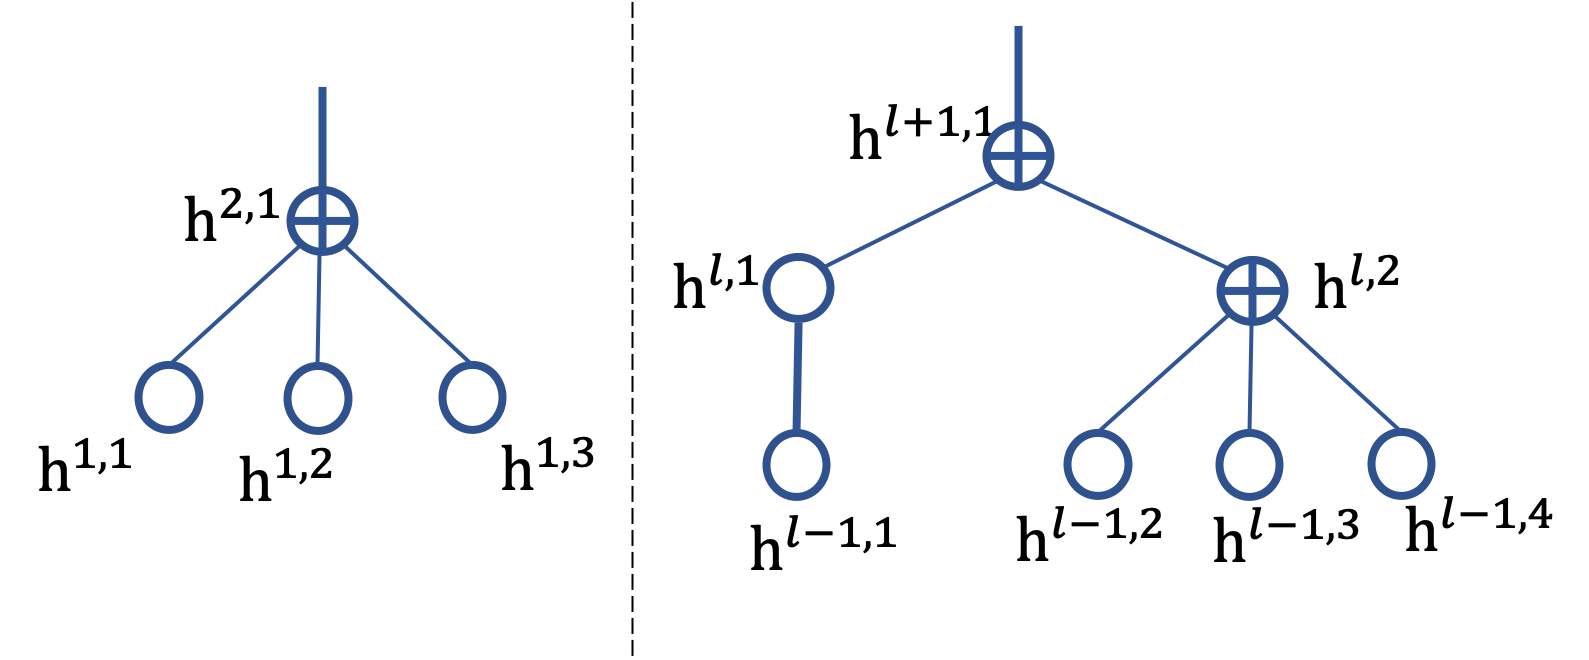
\includegraphics[width=1.0\linewidth]{fig/tree_node.png}
\end{center}
\vspace{-0.15in}
\caption{\small  (Left)  Node $\mathbf{h}^{2, 1}$ connects its children with invertible functions. Messages from the children are aggregated at the parent, $\mathbf{h}^{2,1}$. (Right) An illustration of the latent structure from layer $l-1$ to $l+1$.  $\oplus$ is an aggregation node, and circles stand for non-aggregation~nodes. }
\label{fig:tree}
\vspace{-0.1in}
\end{wrapfigure}

Figure~\ref{fig:tree}-Right gives an illustration of a tree structure induced by variational flow graphical model.  There are two types of nodes in a VFG: \emph{aggregation} nodes and \emph{non-aggregation} nodes. 
A non-aggregation node connects other nodes with a single flow function or an identity function. An aggregation node has multiple children, and it can only connect with each of its children with an identity function. 

The hierarchical generative network comprises $L$ layers, $\mathbf{h}^l$ denotes the latent variable in layer $l$, and $\theta$ is the vector of model parameters. We use $\mathbf{h}^{l, i}$ to denote the $i$th node's latent variable  in layer $l$, and $\mathbf{h}^{(j)}$ to represent node $j$'s latent variable without specification of the layer number, and $j$ is the node index on a tree or graph.  
The joint distribution of the hierarchical model is given by:
 {\small
\begin{align}\notag %\label{eq:joint}
p_{\theta}(\mathbf{x}, \mathbf{h}) = p( \mathbf{h}^{L}) p(\mathbf{h}^{L-1} | \mathbf{h}^{L}) \cdot \cdot  \cdot p(\mathbf{h}^{1} | \mathbf{h}^{2})  p(\mathbf{x} | \mathbf{h}^{1}) \, .
\end{align}}
where $\mathbf{h}=\{\mathbf{h}^1, \cdots, \mathbf{h}^L \}$ denotes the set of latent variables of the model. The hierarchical prior distribution is given by factorization $p(\mathbf{h}) =  p( \mathbf{h}^{L})\mathbf{\Pi}_{l=1}^{L-1}p(\mathbf{h}^{l} | \mathbf{h}^{l+1}) $.

The probability density function $p(\mathbf{h}^{l-1} | \mathbf{h}^{l})$ in the prior is modeled with one or multiple invertible normalizing flow functions. In the following sections of this paper, identity function is considered as a special case of flow functions, and its inverse is itself.  We follow the variational inference approach to approximate the posterior distribution of latent variables. 
The hierarchical posterior~(recognition network) is factorized as
 {\small
 \begin{align}\label{eq:posterior}
q_{\theta}(\mathbf{h}| \mathbf{x}) =  q(\mathbf{h}^1 | \mathbf{x})  q(\mathbf{h}^2 | \mathbf{h}^1) \cdot \cdot  \cdot  q(\mathbf{h}^{L} | \mathbf{h}^{L-1}).
\end{align}}
%\vspace{-0.1in}
Evaluation of the posterior~\eqref{eq:posterior} involves information flows from the bottom of the tree to the top, and similarly, computation of the prior takes the reverse direction. By leveraging the hierarchical conditional independence in both the prior and  posterior,  the ELBO regarding the model is given by  {\small
\begin{align} \label{eq:elbo}
    \log p_{\theta}(\mathbf{x})
    \geqslant & \mathcal{L}(\mathbf{x}; \theta) 
    = \mathbb{E}_{q(\mathbf{h}^{1:L}|\mathbf{x})}\big[ \log p(\mathbf{x}|\mathbf{h}^{1:L})  \big] - \sum_{l=1}^{L} \mathbf{KL}^l.
%\vspace{-0.2in}
\end{align}}
Here $\mathbf{KL}^l$ is the Kullback-Leibler divergence between the posterior and prior in layer $l$. The first term in~(\ref{eq:elbo}) evaluates data reconstruction.  % from the bottom  layerfrom the top layer
When $1\leqslant l \leqslant L$, 
 {\small
\begin{align} \label{eq:kl}
\mathbf{KL}^l 
=\mathbb{E}_{q(\mathbf{h}^{1:L}|\mathbf{x})}\big[  \log q(\mathbf{h}^{l}|\mathbf{h}^{l-1})   - \log p(\mathbf{h}^{l}|\mathbf{h}^{l+1}) \big].
\end{align}}
When $l=L$, 
$\mathbf{KL}^L =  \mathbb{E}_{q(\mathbf{h}^{1:L}|\mathbf{x})}\big[  \log q(\mathbf{h}^{L}|\mathbf{h}^{L-1})- \log p(\mathbf{h}^{L})  \big].$



%\vspace{-0.1in}
\subsection{ Aggregation Nodes}\label{sec:node_aggr}
\begin{wrapfigure}{r}{0.4\textwidth}
\vspace{-0.6in}
\begin{center}
 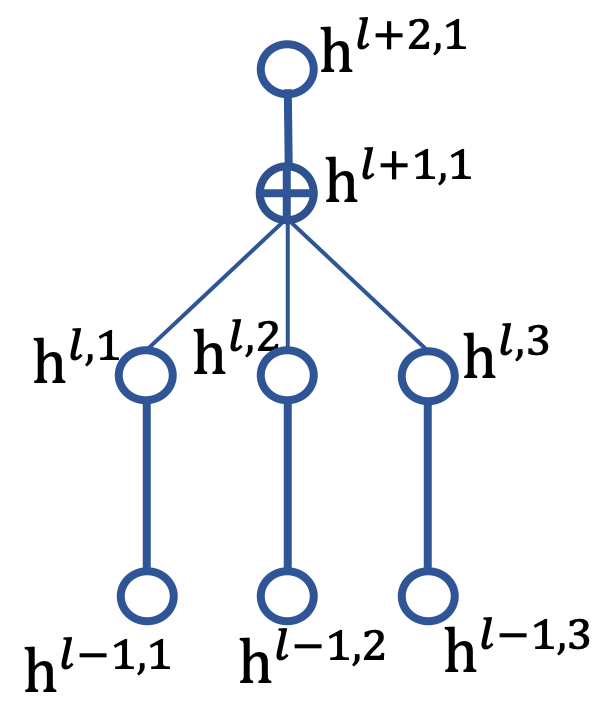
\includegraphics[width=1in]{fig/aggre_node.png}
  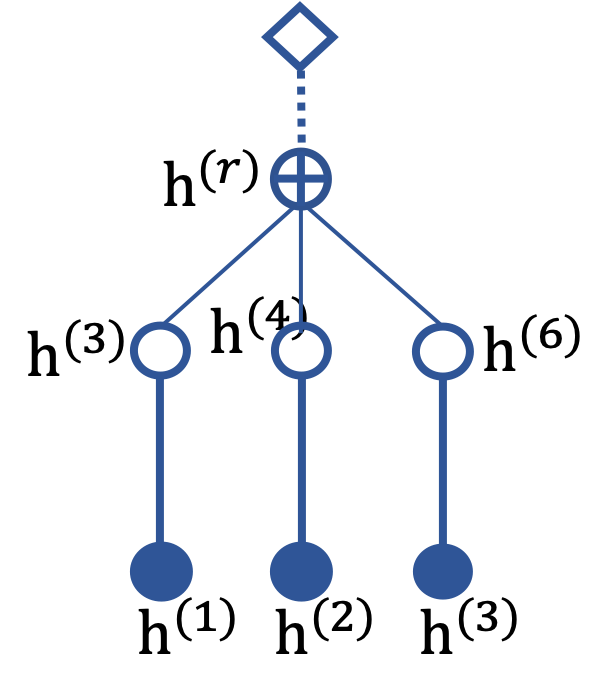
\includegraphics[width=1in]{fig/aggre_model.png}
\end{center}
   \caption{(Left) Aggregation node $\mathbf{h}^{l+1,1}$ has three children, $\mathbf{h}^{l,1}$, $\mathbf{h}^{l,2}$, and $\mathbf{h}^{l,3}$. Thin lines are identity functions, and thick lines are flow functions. (Right) A VFG model with one aggregation node, $\mathbf{h}^{(r)}$. Solid circles are nodes with observed values, and the diamond is the prior for the root node.}
\label{fig:node_aggre}
\vspace{-0.1in}
\end{wrapfigure}
 There are two approaches to aggregate signals from different nodes:  average-based and concatenation-based.
 We rather focus on average-based aggregation in this paper,  and Figure~\ref{fig:node_aggre}-Left gives  an example denoted by the operator $\oplus$. 
As mentioned above, we take  an identity function as a special case of flow functions, and its inverse is itself.
Let $\mathbf{f}_{(i, j)}$ be the direct edge~(function) from node $i$ to node $j$, and $\mathbf{f}^{-1}_{ (i, j)}$ or  $\mathbf{f}_{ (j, i)}$ defined as its inverse function. Then, we observe that at node $i$
 {\small
 \begin{align*}
&  \mathbf{h}^{(i)} = \frac{1}{|ch(i)|} \sum_{j \in ch(i) } \mathbf{f}_{(j,i)}(\mathbf{h}^{(j)})  , \\ &\widehat{\mathbf{h}}^{(i)} = \frac{1}{|pa(i)|} \sum_{j \in pa(i) } \mathbf{f}^{-1}_{ (i,j)}(\widehat{\mathbf{h}}^{(j)}) \, .
\end{align*}} 
Notice that the above two equations hold even when node $i$ has only one child or parent.
In the sequel, we consider that all latent variables, noted $\mathbf{h}^{l, i}$, for all $l \in [L]$ and $i \in \mathbb{N}$, are distributed according to Laplace distributions. 
With the identity function between the  parent and its children, there are two aggregation rules regarding an average aggregation node: (a) the parent value is the mean of its children, i.e., $\mathbf{h}^{(i)} = \frac{1}{|ch(i)|} \sum_{j \in ch(i)} \mathbf{h}^{(j)}$; (b) the  child node have the same reconstruction value than its parent, i.e., $\widehat{\mathbf{h}}^{(j)} = \widehat{\mathbf{h}}^{(i)}, \forall j \in ch(i)$. 


We use Figure~\ref{fig:node_aggre}-Right as an example to illustrate a simple model that  has only one average aggregation node. Then (\ref{eq:elbo}) yields the ELBO,
 {\small
\begin{align}  \label{eq:one_agg_node}
\log p(\mathbf{x})   \geqslant  \mathcal{L}(\mathbf{x}; \theta)=& \mathbb{E}_{q(\mathbf{h} | \mathbf{x})} \big[\log p(\mathbf{x}|\widehat{\mathbf{h}}^1)\big] -\mathbb{E}_{q(\mathbf{h} | \mathbf{x})} \big[\log q(\mathbf{h}^1 | \mathbf{x}) -\log p(\mathbf{h}^1|\widehat{\mathbf{h}}^2)\big] \\ \notag
&- \textbf{\text{KL}}\big(q(\mathbf{h}^2 | \mathbf{h}^1) | p(\mathbf{h}^2)\big).
\end{align}} 
From  Figure~\ref{fig:node_aggre}-Right,  $\mathbf{h}^{(r)}$ is the root, and it has $k$ children, $\mathbf{h}^{(t)}, t = 1,...,k$, and $k=3$. 
With $\mathbf{f}_t$ as the flow function connecting $\mathbf{h}^{(t)}$ and $\mathbf{x}^{(t)}$, according to the aggregation rules, we get:
 {\small
\begin{equation}
\begin{split}
& \mathbf{h}^{(t)} = \mathbf{f}_t(\mathbf{x}^{(t)})\, ,\quad  \widehat{\mathbf{h}}^{(r)} = \mathbf{h}^{(r)} = \frac{1}{k}\sum_{t=1}^k \mathbf{h}^{(t)} , \quad \widehat{\mathbf{h}}^{(t)}= \widehat{\mathbf{h}}^{(r)}, \ t = 1,...,k \, .
 \end{split}
 \end{equation}}
 Assume the data to be normally distributed, then 
 {\small
\begin{align}\notag
 &\log p(\mathbf{x}|\widehat{\mathbf{h}}^1) 
 =-\sum_{t=1}^k\bigg\{ \underbrace{\frac{1}{2\sigma^2_{\mathbf{x}}}\big|\big| \mathbf{x}^{(t)} - \mathbf{f}_t^{-1}(\widehat{\mathbf{h}}^{(r)})\big|\big|_2^2 }_{\textrm{By} \  \widehat{\mathbf{x}}^{(t)}=\mathbf{f}_t^{-1}(\widehat{\mathbf{h}}^{(t)})=\mathbf{f}_t^{-1}(\widehat{\mathbf{h}}^{(r)})} \bigg\}+C , \  \log p(\mathbf{h}^1|\widehat{\mathbf{h}}^2) = -\sum_{t=1}^k\big\{ \underbrace{\big|\big|  \mathbf{f}_t(\mathbf{x}^{(t)}) - \widehat{\mathbf{h}}^{(r)}\big|\big|_1}_{\textrm{By} \  \widehat{\mathbf{h}}^{2}= \widehat{\mathbf{h}}^{(r)}, \  \mathbf{h}^{(t)} = \mathbf{f}_t(\mathbf{x}^{(t)})} \big\} +C .
 \end{align} 
 }
 Here $\sigma_{\mathbf{x}}$ is a constant standard deviation. 
We notice that maximizing the ELBO, or minimizing the $\mathbf{KL}$ term of an aggregation node will force the model to satisfy aggregation rule (b). 
  \begin{wrapfigure}{rI}{0.5\textwidth}
 \vspace{-0.1in}
\begin{minipage}{0.5\textwidth}
\begin{algorithm}[H]
 {\footnotesize
   \caption{Inference model parameters with  forward and backward message propagation}
   \label{alg:main}
\begin{algorithmic}[1]
%\SetCustomAlgoRuledWidth{0.45\textwidth}
   \STATE {\bfseries Input:} Data distribution $\mathcal{D}$,  $\mathcal{G} = \{\mathcal{V}, \mathbf{f}\}$
   \FOR {$s=0,1,...$} 
   \STATE  Sample minibatch $b$ samples $\{\mathbf{x}_1, ..., \mathbf{x}_b \}$ from $\mathcal{D}$;
   \FOR{$i \in \mathcal{V}$}\label{line:for2}
    \STATE  \textcolor{blue}{// forward message passing}
   \STATE $\mathbf{h}^{(i)} = \frac{1}{|ch(i)|} \sum_{j \in ch(i) } \mathbf{f}_{(j,i)}(\mathbf{h}^{(j)})$; \label{line:forward} 
    \ENDFOR
    \STATE $\widehat{\mathbf{h}}^{(i)} = \mathbf{h}^{(i)} \ \  \text{if} \ i \in \mathcal{R}_{\mathcal{G}} $ or $i \in$ layer L;
   \FOR{$i \in \mathcal{V}$}
   \STATE \textcolor{blue}{// backward message passing}
   \STATE $\widehat{\mathbf{h}}^{(i)} = \frac{1}{|pa(i)|} \sum_{j \in pa(i) } \mathbf{f}^{-1}_{ (i,j)}(\widehat{\mathbf{h}}^{(j)}) $;\label{line:backward}  
   \ENDFOR
    \STATE  $\mathbf{h} =  \{\mathbf{h}^{(t)} \big |  t \in \mathcal{V} \}$, $\widehat{\mathbf{h}} =  \{\widehat{\mathbf{h}}^{(t)} \big | t \in \mathcal{V} \}$;
    \STATE Approximate the $\mathbf{KL}$ terms in ELBO for each layer with b samples;
    \STATE Updating VFG model $\mathcal{G}$ with gradient ascending: $\theta^{(s+1)}_{\mathbf{f}} = \theta^{(s)}_{\mathbf{f}} + \nabla_{\theta_{\mathbf{f}}}\frac{1}{b} \sum_{i=1}^b  \mathcal{L}(\mathbf{x}_b; \theta^{(s)}_{\mathbf{f}})   \, .$\label{line:update} 
   \ENDFOR
\end{algorithmic}
}
\end{algorithm}
\end{minipage}
 \vspace{-0.4in}
\end{wrapfigure}
 \vspace{-0.2in}
\section{Algorithms and Implementation}\label{sec:algrithm}

In this section, we develop the training algorithm, see Algorithm~\ref{alg:main}, that outputs the fitted vector of parameters resulting from the maximization of the ELBO objective function~(\ref{eq:elbo}) or~(\ref{eq:elbo_dag}) depending on what graph structure is used.
In Algorithm~\ref{alg:main}, the inference of the latent variables is performed via forwarding message passing, cf. Line~6, and their reconstructions are computed in backward message passing, cf. Line~11.

Unlike Variational Autoencoders (VAE), the variance of latent variables in a VFG is approximated rather than parameterized with neural networks. 
A VFG is a deterministic network passing latent variable values between nodes. 
The reconstruction~(likelihood) terms in each layer are computed with forward and backward node states. 
Ignoring explicit neural network parameterized variances for all latent nodes enables us to use flow-based models as both the encoders and decoders. 
We thus obtain a deterministic ELBO objective~(\ref{eq:elbo})-~(\ref{eq:elbo_dag}) that can efficiently be optimized with standard stochastic optimizers. 

 \begin{wrapfigure}{r}{0.5\textwidth}
 \vspace{-0.7in}
\begin{minipage}{0.5\textwidth}
\begin{algorithm}[H]
 {\footnotesize
%\algsetup{indent=0.25em}
   \caption{Inference model parameters with random masking}
   \label{alg:rand_mask}
\begin{algorithmic}[1]
   \STATE {\bfseries Input:} Data distribution $\mathcal{D}$,  $\mathcal{G} = \{\mathcal{V}, \mathbf{f}\}$
   \FOR {$s=0,1,...$}
   \STATE  Sample minibatch $b$ samples $\{\mathbf{x}_1, ..., \mathbf{x}_b \}$ from $\mathcal{D}$;
   \STATE  
    % Optimize~(\ref{eq:elbo}) with steps~\ref{line:for2} to~\ref{line:update} in Algorithm~\ref{alg:main};
    Optimize~(\ref{eq:elbo}) with Line~4 to Line~15 in Algorithm~\ref{alg:main};
    \STATE  Sample a subset of the $k$ data sections as data observation set $O_{\mathbf{x}}$; $O \leftarrow O_{\mathbf{x}}$;
   \FOR{$i \in \mathcal{V}$}
    \STATE  \textcolor{blue}{// forward message passing}
   \STATE $\mathbf{h}^{(i)} = \frac{1}{|ch(i) \cap O |} \sum_{j \in ch(i) \cap O} \mathbf{f}_{(j,i)}(\mathbf{h}^{(j)})$; 
     \STATE  $O \leftarrow O \cup \{i\}$ if $ch(i) \cap O \neq \emptyset $; 
    \ENDFOR
    \STATE $\widehat{\mathbf{h}}^{(i)} = \mathbf{h}^{(i)} \ \  \text{if} \ i \in \mathcal{R}_{\mathcal{G}} $ or $i \in$ layer L;
   \FOR{$i \in \mathcal{V}$}
   \STATE \textcolor{blue}{// backward message passing}
   \STATE $\widehat{\mathbf{h}}^{(i)} = \frac{1}{|pa(i)|} \sum_{j \in pa(i) } \mathbf{f}^{-1}_{ (i,j)}(\widehat{\mathbf{h}}^{(j)}) $;%\label{line:backward}  
   \ENDFOR
    \STATE  $\mathbf{h} =  \{\mathbf{h}^{(t)} \big |  t \in \mathcal{V} \cap O \}$, $\widehat{\mathbf{h}} =  \{\widehat{\mathbf{h}}^{(t)} \big | t \in \mathcal{V} \}$;
    \STATE Approximate the $\mathbf{KL}$ terms in ELBO for each layer with b samples;
    \STATE Updating VFG with gradient of~(\ref{eq:elbo_tree_mask}): $\theta^{(s+1)}_{\mathbf{f}} = \theta^{(s)}_{\mathbf{f}} + \nabla_{\theta_{\mathbf{f}}}\frac{1}{b} \sum_{i=1}^b  \mathcal{L}(\mathbf{x}_b, O_{\mathbf{x}}; \theta^{(s)}_{\mathbf{f}})   \, ,$
   %\ENDFOR 
   \ENDFOR
\end{algorithmic}
}
\end{algorithm}
\end{minipage}
 \vspace{-0.3in}
\end{wrapfigure}

\subsection{Layer-wise Training}
From a practical perspective, layer-wise training strategy can improve the efficiency of a model especially when it is constructed of more than two layers. 
In such a case, the parameters of only one layer are updated with backpropagation of the gradient of the loss function while keeping the other layers fixed at each optimization step. 
By maximizing the ELBO~(\ref{eq:elbo}) or~(\ref{eq:elbo_dag}) with the above algorithm, the aggregation rules in Section~\ref{sec:node_aggr} are expected to be satisfied. 
We can improve the inference on sub-graphs discussed in Section~\ref{sec:infer} by using the random masking method introduced in the sequel.

%\vspace{-0.2in}
\subsection{Random Masking}
Inference on a VFG model requires the aggregation node's state to be imputed from observed children's state, as shown in~(\ref{eq:aggr_obs_ch}).
Then, unobserved children's state can be inferred from their parent.  
The inference ability of VFG via imputation can be reinforced by \emph{masking out} some sections of the training samples. 
The training objective can be changed to force the model to impute the value of the masked sections. 
For example in a tree model, the alternative objective function reads
{\small
\begin{align}  \label{eq:elbo_tree_mask}
\mathcal{L}(\mathbf{x}, O_{\mathbf{x}}; \theta)
= & \sum_{t: 1\leqslant t \leqslant k, t\notin O}
 \mathbb{E}_{q(\mathbf{h}^{1}|\mathbf{x}^{O_{\mathbf{x}}} )} \bigg[ \log p( \mathbf{x}^{(t)}|  \widehat{\mathbf{h}}^{1})   \bigg] \\ \notag
 &- \sum_{l=1}^{L-1}  \mathbb{E}_{q(\mathbf{h}|\mathbf{x})} \bigg[ \log q(\mathbf{h}^{l}|\mathbf{h}^{l-1}) - \log p( \mathbf{h}^{l}|  \widehat{\mathbf{h}}^{l+1})   \bigg]    
 -  \textbf{\text{KL}}\big(q(\mathbf{h}^L | \mathbf{h}^{L-1} )   | p(\mathbf{h}^L)  \big).
\end{align} }
where $O_{\mathbf{x}}$ is the index set of leaf nodes  with observation, and $\mathbf{x}^{O_{\mathbf{x}}}$ is the union of observed data sections. 
Considering a minibatch of training samples, the objectives function in~(\ref{eq:elbo})
and~(\ref{eq:elbo_tree_mask}) can thus be optimized sequentially. 
The training with \emph{random masking} is described in Algorithm~\ref{alg:rand_mask}. 

%\vspace{-0.2in}
\section{Inference on VFG Models }\label{sec:infer}

%\subsection{Inference on Trees }
\begin{wrapfigure}{r}{0.5\textwidth}
\vspace{-0.5in}
\begin{center}
 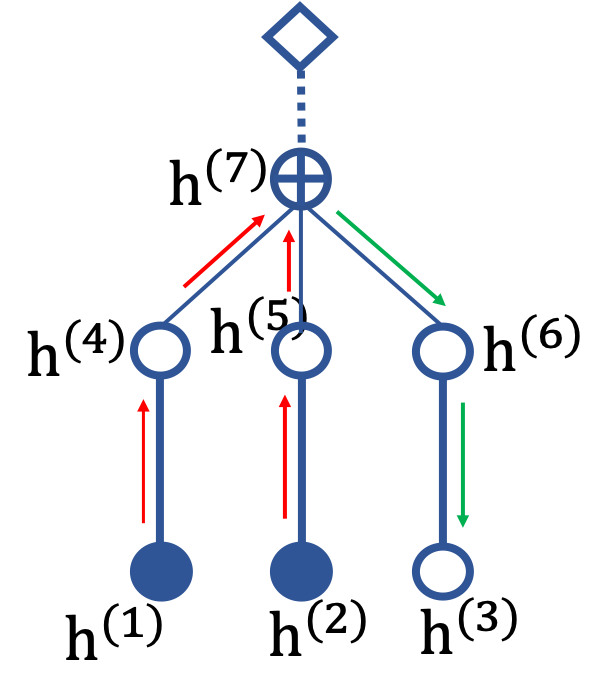
\includegraphics[width=0.32\linewidth]{fig/two_layer_infer.png}
 %\hspace{0.15in}
 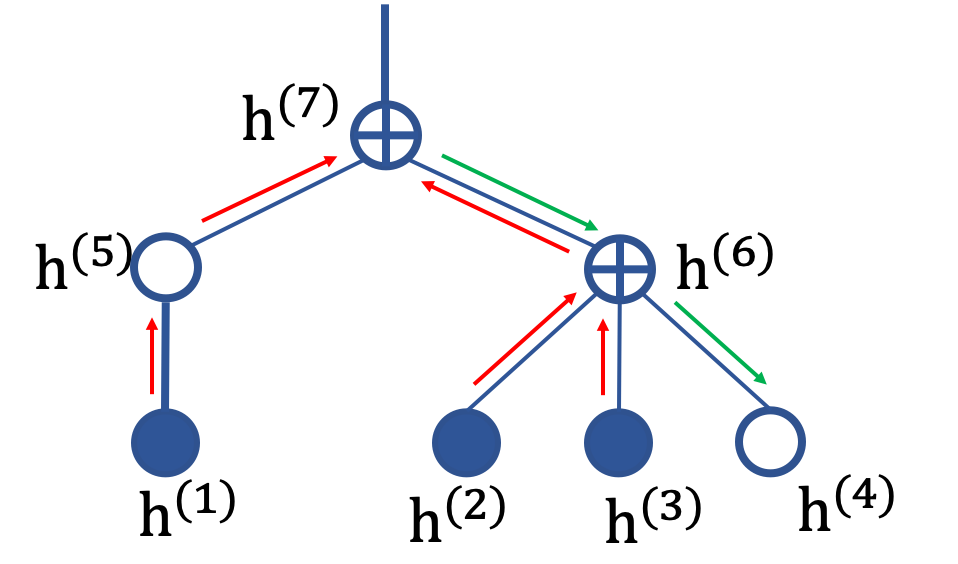
\includegraphics[width=0.62\linewidth]{fig/tree_infer.png}
\end{center}
\vspace{-0.1in}
 \caption{{\small (Left) Inference on model with single aggregation node. Node 7 aggregates information from node 1 and 2, and  pass down the updated state to node 3 for prediction. (Right) Inference on a tree model. Observed node states are gathered at node 7 to predict the state of node 4. Red and green lines are forward and backward messages, respectively.}}
\label{fig:two_layer_infer}
\vspace{-0.1in}
\end{wrapfigure}

Given a trained VFG model, our goal in this subsection is to infer the state of any node given observed ones. 
Relations between variables at different nodes can also be inferred via our flow-based graphical model. 
The hidden state of the parent node $j$ in a single aggregation model can be approximated by the observed children as follows:
 {\small
 \begin{align}\label{eq:aggr_obs_ch}
\mathbf{h}^{(j)}  = \frac{1}{|ch(j) \cap O|}\sum_{i \in ch(j) \cap O} \mathbf{h}^{(i)} \, ,
\end{align}}
where $O$ is the set of observed leaf nodes, see Figure~\ref{fig:two_layer_infer}-left for an illustration. 
Observe that for either a tree or a DAG, the state of any given node is updated via messages received from its children. Figure~\ref{fig:two_layer_infer} illustrates this inference mechanism for trees in which the structure enables us to perform message passing among the nodes. 
We derive the following Lemma establishing the relation between two leaf nodes:
%\color{red}{wrong}
\begin{lemma}\label{lm:apprx}
Let $\mathcal{G}$ be a trained variational flow graphical model (with a tree structure) with $L$ layers, and $i$ and $j$ are two leaf nodes with $a$ as the closest common ancestor. Given observed value at node $i$, the value of node $j$ can be approximated by   $\widehat{\mathbf{x}}^{j} \approx  \mathbf{f}_{(a,j)}(\mathbf{f}_{(i, a)}(\mathbf{x}^{(i)}))$. Here $\mathbf{f}_{(i, a)}$ is the flow function path from node $i$ to node $a$. The conditional density of $\mathbf{x}^{(j)}$ given $\mathbf{x}^{(i)}$ can be approximated by: 
 {\small
\begin{align} \label{eq:cond_llk}
& \log p(\mathbf{x}^{(j)} | \mathbf{x}^{(i)}) 
\approx  \log p(\widehat{\mathbf{h}}^L) -  \frac{1}{2} \log \big(\det \big(\mathbf{J}_{\widehat{\mathbf{x}}^{(j)}}(\widehat{\mathbf{h}}^L)^\top\mathbf{J}_{\widehat{\mathbf{x}}^{(j)}}(\widehat{\mathbf{h}}^L)\big) \big).
\end{align}}
\end{lemma}
Considering the normalizing flow~(\ref{eq:flow}), we have the following identity for each node of the graph structure:
 {\small
\begin{align*}
p(\mathbf{h}^{(i)} | \mathbf{h}^{pa(i)}) & = p(\mathbf{h}^{pa(i)}) \big|\det(\frac{\partial \mathbf{h}^{pa(i)} }{\partial \mathbf{h}^{(i)}})\big|   =
p(\mathbf{h}^{pa(i)}) \big|\det(\mathbf{J}_{\mathbf{h}^{pa(i)}}(\mathbf{h}^{(i)}))\big| \, .
\end{align*}} 
% The proof of Lemma~\ref{lm:apprx} can be found in the appendix. 

\begin{remark}\label{rmk:apprx_mul}
Let $O$ be the set of observed leaf nodes, $j$ be an unobserved node, and $a$ the closest ancestor of $O \cup \{a\}$. 
Then the state of $j$ can be imputed with $\widehat{\mathbf{x}}^{j} \approx  \mathbf{f}_{(a,j)}(\mathbf{f}_{(O, a)}(\mathbf{x}^{(i)}))$, where $\mathbf{f}_{(O, a)}$ is the flow function path from all nodes in $O$ to $a$.
Note that approximation~(\ref{eq:cond_llk}) still holds for $p(\mathbf{x}^{(j)} | \mathbf{x}^{O})$.
\end{remark}
%Those results can naturally be extended to DAGs.

\vspace{-0.1in}
\section{Numerical Experiments}\label{sec:numerical}
%We present in this section several numerical experiments to highlight the benefits of our VFG model.
The first main application we present is the imputation of missing values. We compare our method with several baseline models  on a synthetic dataset.
The second application we present is the task of learning the disentangled latent representations that separate the explanatory factors of variations in the data, see~\cite{bengio2013representation}.
For that latter application, the model is trained and evaluated on the MNIST handwritten digits dataset.



%\vspace{-0.05in}
\subsection{Evaluation on Inference with Missing Entries Imputation}%\label{sec:exp:mnist}
%\vspace{-0.05in}
We now focus on the task of imputing missing entries in a graph structure.
For all the following experiments, the models are trained on the training set and are used to infer the missing entries of samples in the testing set. We use MSE  regarding the prediction and ground truth as the imputation metric in the comparison of different methods. 

\textbf{Baseline Methods:} We use the following baselines for data imputation:\vspace{-0.05in}
\begin{itemize}
\item \textit{Mean Value:} Using training set mean values to replace the missing entries in the testing set.   
\item \textit{Iterative Imputation:} A strategy for imputing missing values by modeling each feature with missing values as a function of other features in a Round-Robin fashion.   
% We choose the KNeighborRegressor as the specific function~\cite{scikit-learn}.
%\vspace{-0.1in}
\item \textit{KNN:} To use K-Nearest Neighbor for data imputation,  we compare the non-missing entries of each sample to the training set and use the  average of top $k$ samples as imputation values   
%\vspace{-0.1in}
\item \textit{Multivariate Imputation by Chained Equation (MICE):} This method impute the missing entries with multiple  rounds of inference. This method can handle different type of data.
\end{itemize}  
\textbf{Synthetic dataset: } In this set of experiments, we study the proposed model with synthetic datasets.
We generate $10$ synthetic datasets (using different seeds) of $1\,300$ data points, $1\,000$ for the training phase of the model, $300$ for imputation testing. 
\begin{wrapfigure}{r}{0.3\textwidth}
    \centering
       \includegraphics[width=0.35\textwidth]{fig/sim_box_t.eps}
%   \includegraphics[width=1.6in]{fig/sim_elbo.eps}
    \captionof{figure}{Synthetic datasets: MSE boxplots of VFG and baseline methods.}
    \label{fig:sim}
\end{wrapfigure}
Each data sample  has $8$ dimensions with $2$ latent variables. 
Let $z_1 \sim \mathcal{N}(0,1.0^2)$ and $z_2 \sim  \mathcal{N}(1.0,2.0^2)$ be the latent variables. For a sample $\mathbf{x}$, we have  $x_1=x_2 = z_1, x_3=x_4= 2\textrm{sin}(z_1), x_5=x_6 =z_2$, and $x_7= x_8 = z_2^2$.  In the testing dataset, $x_3$, $x_4$, $x_7$, and $x_8$ are missing. We use a VFG model with a single average aggregation node that has four children, and each child connects the parent with a flow function consisting of 3 coupling layers~\cite{Dinh2016DensityEU}. 
Each child takes 2 variables as input data section, and the latent dimension of the VFG is $2$.
We compare, Figure~\ref{fig:sim}, our VFG method with the baselines described above using boxplots on MSE errors for those $10$ simulated datasets.
We can see that the proposed VFG model performs much better than mean value, iterative, and MICE methods. 
VFG achieves similar MSE values but with much smaller performance variance compared with KNN methods.  

\subsection{ELBO and Likelihood}\label{sec:exp:elbo}

In Table~\ref{tab:elbo}, the negative evidence lower bound~(-ELBO) and the estimated negative likelihood~(NLL) for baseline methods on three datasets, MNIST, Caltech101, and Omniglot. The results of the baseline methods are from~\cite{berg2018sylvester}. These methods are VAE based methods  enhanced with  normalizing flows.  They use 16 flows to improve the posterior estimation. SNF is orthogonal sylvester flow method with a bottleneck of M = 32. We set the VFG coupling block number with  two different values, and they achieve similar performance. Compared to VAE based methods, the proposed VFG model can achieve significant improvement on both ELBO and NLL values.


\begin{center}
{\footnotesize
\begin{tabular}{l | c  c   c  c  c  c }
\hline
 \multirow{2}{0nc}{\textbf{Model}} & \multicolumn{2}{c}{\textbf{MNIST}} & \multicolumn{2}{c}{\textbf{Caltech101}} & \multicolumn{2}{c}{\textbf{Omniglot}} \\
 %\hline 
 & -ELBO & NLL  &  -ELBO & NLL  & -ELBO & NLL  \\
\hline
 VAE~\cite{kingma2013auto} & 86.55 $\pm$ 0.06  & 82.14 $\pm$ 0.07& 110.80 $\pm$ 0.46 & 99.62 $\pm$ 0.74 & 104.28 $\pm$ 0.39 & 97.25 $\pm$ 0.23 \\
Planer~\cite{rezende2015variational} & 86.06 $\pm$ 0.31 & 81.91 $\pm$ 0.22 & 109.66 $\pm$ 0.42 & 98.53 $\pm$ 0.68 & 102.65 $\pm$ 0.42 & 96.04 $\pm$ 0.28 \\
IAF~\cite{kingma2016improving} & 84.20 $\pm$ 0.17& 80.79 $\pm$ 0.12 & 111.58 $\pm$ 0.38 & 99.92 $\pm$ 0.30 & 102.41 $\pm$ 0.04 & 96.08 $\pm$ 0.16 \\
SNF~\cite{berg2018sylvester} & 83.32 $\pm$ 0.06 & 80.22 $\pm$ 0.03 & 104.62 $\pm$ 0.29 & 93.82 $\pm$ 0.62 & 99.00 $\pm$ 0.04 & 93.77 $\pm$ 0.03 \\
\hline
VFG~(b=4) &\textbf{74.01} & \textbf{67.58} & \textbf{67.2} & \textbf{65.9}  &\textbf{84.29} & \textbf{83.11}\\  
%VFG~(b=6) & \textbf{73.21} &  67.74\\ 
\hline
\end{tabular}
\captionof{table}{Negative log-likelihood and free energy (negative evidence lower bound) for static MNIST, Caltech101, and Omniglot.}
\label{tab:elbo}
}
\end{center}


\subsection{Latent Representation Learning on MNIST}\label{sec:exp:mnist}
%\vspace{-0.05in}
\begin{wrapfigure}{r}{0.45\textwidth}
    \centering
       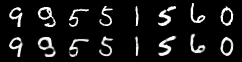
\includegraphics[width=0.45\textwidth]{fig/reconst_Y.png}
%   \includegraphics[width=1.6in]{fig/sim_elbo.eps}
        \captionof{figure}{(Top row) original MNIST digits. (Bottom row) reconstructed images using VFG.}
    \label{fig:reconst}
\vspace{-0.12in}
\end{wrapfigure}
In this set of experiments, we evaluate  Variational Flow Graphical Models on latent representation learning of the MNIST dataset~\cite{Lecunmnist2010}. 
We construct a two layer VFG model,  and set $\lambda=1$. 
The first layer consists of one aggregation node with four children, and each child has an input dimension $14\times 14$. 
The second layer is a single flow model.
The latent dimension for this model is $196$. 
Following~\cite{Sorrenson2020}, the VFG model is trained with image labels to improve the disentanglement of the latent representation of the input data. 
Based on the theoretical result introduced in Section~\ref{sec:theory}, we set the parameters of $\mathbf{h}^L$'s prior distribution as a function of image label, i.e., $\lambda^L(u)$, where $u$ denotes the image label. In practice, we use $10$ trainable $\lambda^L$s regarding the $10$ digits. 
The images in the second row of Figure~\ref{fig:reconst} are reconstructions of MNIST samples extracted from the testing set, displayed in the first row of the same Figure, using our proposed VFG model.  

\begin{minipage}{\textwidth}
  \begin{minipage}[b]{0.49\textwidth}
  \begin{figure}[H]
    \centering
       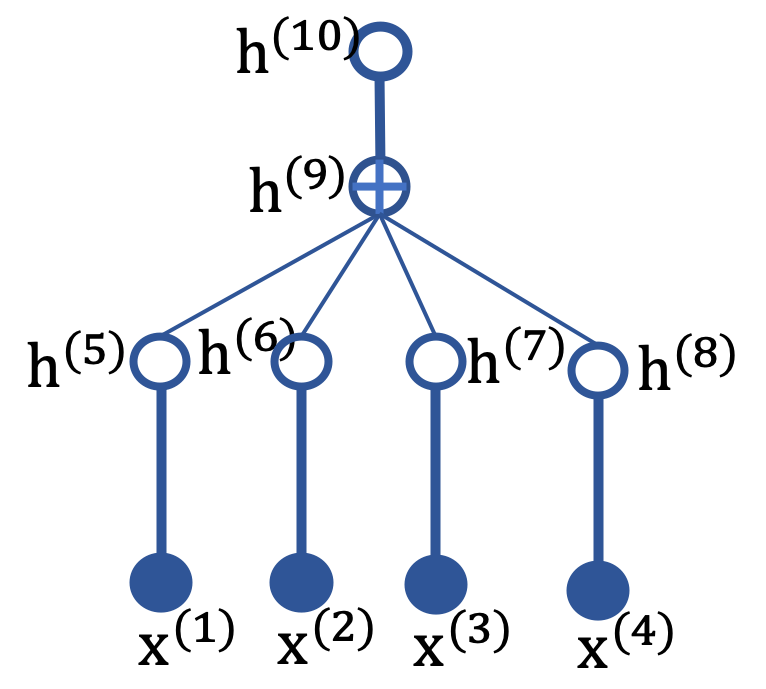
\includegraphics[width=0.6\textwidth]{fig/tree_mnist.png}
    \captionof{figure}{The tree structure for MNIST.}
    \label{fig:struct}
\end{figure}
  \end{minipage}
  \hfill
  \begin{minipage}[b]{0.49\textwidth}
\begin{figure}[H]
    \centering
       \includegraphics[width=0.6\textwidth]{fig/z_Y.eps}
%   \includegraphics[width=1.6in]{fig/sim_elbo.eps}
        \captionof{figure}{MNIST: t-SNE plot of latent variables from VFG learned with labels.}
    \label{fig:z_tsne}
%\vspace{-0.15in}
\end{figure}
\end{minipage}
\end{minipage}

Figure~\ref{fig:z_tsne} shows the t-distributed stochastic neighbor embedding (t-SNE)~\cite{maaten2008visualizing} plot of $2,000$ testing images's latent variables learned with our model, and $200$ for each digit. 
We observe from Figure~\ref{fig:z_tsne}, that VFG can learn separated latent representations to distinguish different hand-written numbers.

\vspace{-0.1in}
\section{Conclusion}\label{sec:conclusion}
\vspace{-0.05in}
In this paper, we propose VFG, a variational flow graphical model that aims at bridging the gap between normalizing flows and the paradigm of graphical models.
Our VFG model learns the hierarchical latent structure of the input data through message passing between latent nodes, assumed to be random variable.
The posterior inference, of the latent nodes given input observations, is facilitated by the careful embedding of normalizing flow in the general graph structure, thus bypassing the stochastic sampling step.
Experiments on different datasets illustrate the effectiveness of the model. 
Future work includes applying our VFG model to fine grained data relational structure learning and reasoning. 


\bibliography{ref}
\bibliographystyle{abbrv}


%%%%%%%%%%%%%%%%%%%%%%%%%%%%%%%%%%%%%%%%%%%%%%%%%%%%%%%%%%%%

\appendix


\section{Additional Numerical Experiments}
In all the experiments of the paper, we use the same  coupling block~\cite{Dinh2016DensityEU} to construct different flow functions. 
The coupling block consists in three fully connected layers~(of dimension $64$) separated by two RELU layers along with the coupling trick. 
Each flow function has block number $b\geqslant 2$. 
All latent variables, $\mathbf{h}^{i}, i \in \mathcal{V}$ are forced to be non-negative via Sigmoid or RELU functions. 
Non-negativeness can help the model to identify sparse structures of the latent space. 

\subsection{California Housing Dataset}
We further investigate the method on a real dataset.  
The California Housing~\cite{chsklearn} dataset  has 8 feature entries and $20\,640$ data samples. 
We use the first $20\,000$ samples for training  and $100$ of the rest for testing.  
We get  4 data sections, and each section contains 2 variables. 
In the testing set, the second section is assumed missing for illustration purposes, as the goal is to impute this missing section.
Here, we construct a tree structure VFG with 2 layers. 
The first layer has two aggregation nodes, and each of them has two children. 
The second layer consists of one aggregation node that has two children connecting with the first layer.  
Each flow function has 4 coupling blocks. 
We can see Table~\ref{tab:imp_arrhytmia} that our model yields significantly better results than any other method in terms of prediction error. 
\begin{table}[ht]
\centering
%	\resizebox{\columnwidth}{!}{%
 \begin{tabular}{l | c  }\hline
\textit{Methods} & \textit{Imputation MSE}  \\
\hline
Mean Value &1.993 \\
%\hline
MICE & 1.951\\
%\hline
Iterative Imputation & 1.966\\
%\hline
KNN (k=3) &1.974 \\
%\hline
KNN (k=5) &1.969 \\
\hline
VFG & \textbf{1.356} \\  
\hline
\end{tabular}
%}
\captionof{table}{California Housing dataset: Imputation Mean Squared Error (MSE) results.} \label{tab:imp_arrhytmia}
\end{table}


% \begin{figure}[H]
%     \centering
%       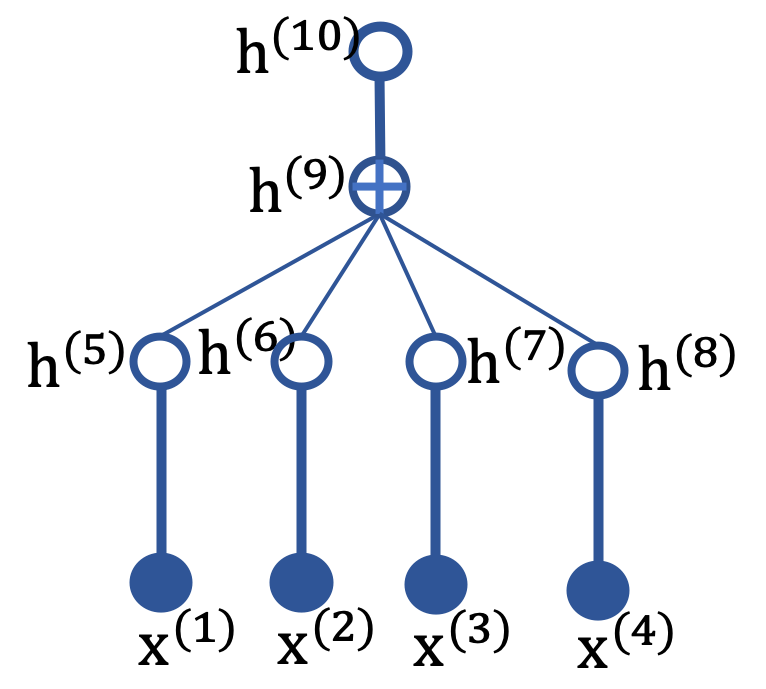
\includegraphics[width=0.3\textwidth]{fig/tree_mnist.png}
%     \captionof{figure}{The tree structure for MNIST.}
%     \label{fig:struct}
% \end{figure}
 
\subsection{Inference on DAGs}
In this set of experiments, we compare VFGs against Bayesian networks and sum-products nets on inference capabilities. 

\subsection{MNIST}
For MNIST, we construct a tree structure VFG model depicted in Figure~\ref{fig:struct}.  
In the first layer, there are 4 flow functions, and each of them takes $14\times 14$ image blocks as the input. 
Thus a $28\times 28$ input image is divided into four $14\times 14$ blocks as the input of VFG model. 
The four nodes are aggregated as the input of the upper layer flow. 


\subsubsection{Latent Representation Learning on MNIST}
Figure~\ref{fig:z_no_Y} presents the t-SNE plot of the root latent variables from VFG trained without labels. The figure clearly shows that even without label information, different digits' representation are roughly scattered in different areas.  Compared to Figure~\ref{fig:z_tsne} in section~\ref{sec:exp:mnist}, label information indeed can improve the latent representation learning. 
\begin{figure}[H]
    \centering
       \includegraphics[width=0.6\textwidth]{fig/z_no_Y_2.eps} 
    \captionof{figure}{MNIST: t-SNE plot of latent variables from VFG learned without labels.}
    \label{fig:z_no_Y}
\end{figure}
 
\subsubsection{Disentanglement on MNIST}
We study disentanglement on MNIST with our proposed VFG model introduced in section~\ref{sec:exp:mnist}. But different from the model in section~\ref{sec:exp:mnist}, here, the distribution parameter $\lambda$ for all latent variables are set to be trainable across all layers.  
Each digit has its trainable vector,  $\lambda \in \mathbb{R}^d$ that is used across all layers. 
To show the disentanglement of learned latent representation, we first obtain the root latent variables of a set of images through forward message passing. Each latent variable's values are changed increasingly within a range centered at the value of the latent variable obtained from last step. 
This perturbation is performed for each image in the set.
Figure~\ref{fig:mnist_dis} shows the change of images by increasing one latent variable from a small value to a larger one. The figure presents some of the latent variables that have obvious effects on images, and most of the $d=196$ variables do not impact the generation significantly. Latent variables $i=6$ and $i=60$ control the digit width. Variable $i=19$ affects the brightness.  $i=92, i=157$ and some of the variables not displayed here control the style of the generated digits. 

\begin{figure}[H]
	\begin{center}

		\mbox{\hspace{-0.15in}	
				\subfigure[i=6, Width]{
				       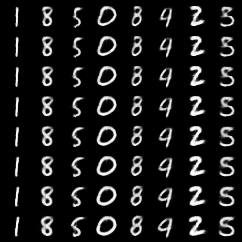
\includegraphics[width=2.2in]{fig/perturb_dim_6.png} 
				}		  
				\subfigure[i=19, Brightness]{
				     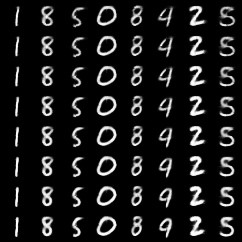
\includegraphics[width=2.2in]{fig/perturb_dim_19.png}
				}		  
								\subfigure[i=60, Upper width]{
				       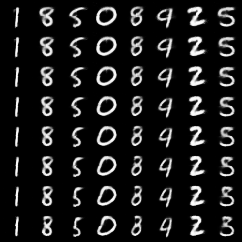
\includegraphics[width=2.2in]{fig/perturb_dim_60.png} 
				}		  
		}

		\mbox{\hspace{-0.15in}	

				\subfigure[i=92]{
				     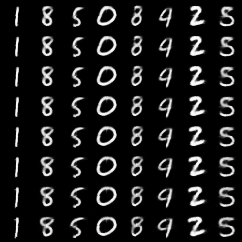
\includegraphics[width=2.2in]{fig/perturb_dim_92.png}
				}		 
				
				\subfigure[i=119, Angle]{
				     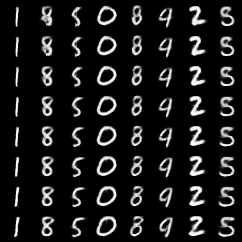
\includegraphics[width=2.2in]{fig/perturb_dim_119.png}
				}		  
								\subfigure[i=157]{
				     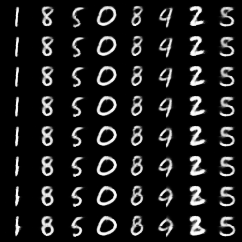
\includegraphics[width=2.2in]{fig/perturb_dim_157.png}
				}		  
		}
	\end{center}
  \captionof{figure}{MNIST: Increasing each latent variable from a small value to a larger one.}\label{fig:mnist_dis}
\end{figure}


%\section{Appendix}
\section{Derivation of the ELBO for both Tree and DAG structures}
\subsection{ELBO of Tree Models}\label{appd:tree_elbo}

Let each data sample has $k$ sections, i.e., $\mathbf{x} = [\mathbf{x}^{(1)}, ..., \mathbf{x}^{(k)}]$. VFGs are graphical models that can integrate different sections or components of the dataset.  We assume that for each pair of connected nodes, the edge is an invertible flow function. 
The vector of parameters for all the edges is denoted by $\theta$. 
The forward message passing starts from $\mathbf{x}$ and ends at $\mathbf{h}^L$, and backward message passing in the reverse direction. We start with the hierarchical generative tree network structure illustrated by an example in Figure~\ref{fig:tree3}. 
Then the marginal likelihood term of the data reads
\begin{align*}
p(\mathbf{x}| \mathbf{\theta}) = \sum_{\mathbf{h}^1, ..., \mathbf{h}^L} p(\mathbf{h}^L | \theta)p(\mathbf{h}^{L-1} | \mathbf{h}^{L},\theta) \cdot \cdot  \cdot  p(\mathbf{x} | \mathbf{h}^{1}, \theta) \, .
\end{align*}

\begin{figure}[H]
    \centering
    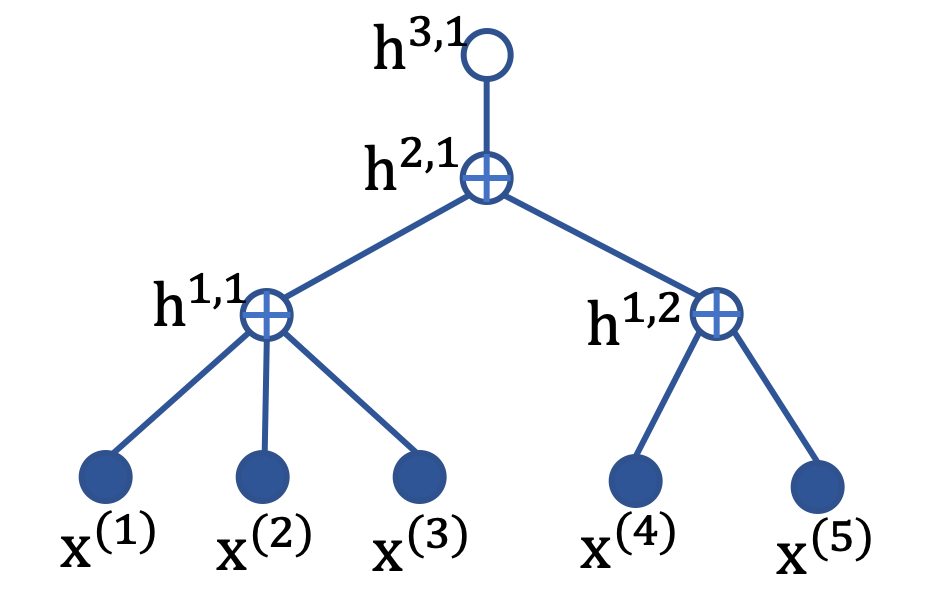
\includegraphics[width=2.3in]{fig/tree3.png}
    \caption{A VFG tree with $L=3$.}
    \label{fig:tree3}
\end{figure}

The hierarchical prior distribution is given by factorization
\begin{align}\label{eq:prior}
p(\mathbf{h}) =  p( \mathbf{h}^{L})\mathbf{\Pi}_{l=1}^{L-1}p(\mathbf{h}^{l} | \mathbf{h}^{l+1}) .
\end{align}
The probability density function $p(\mathbf{h}^{l-1} | \mathbf{h}^{l})$ in the prior is modeled with one or multiple invertible normalizing flow functions. The hierarchical posterior~(recognition network) is factorized as
\begin{align}\label{eq:posterior2}
q_{\theta}(\mathbf{h}| \mathbf{x}) =  q(\mathbf{h}^1 | \mathbf{x})  q(\mathbf{h}^2 | \mathbf{h}^1) \cdot \cdot  \cdot  q(\mathbf{h}^{L} | \mathbf{h}^{L-1}).
\end{align}
Draw samples from the prior~(\ref{eq:prior})
involves sequential conditional sampling from the top of the tree to the bottom, and computation of the posterior~(\ref{eq:posterior2}) takes the reverse direction. Notice that
\begin{align*} %\label{eq:chain}
q(\mathbf{h}| \mathbf{x}) = q(\mathbf{h}^1 | \mathbf{x})  q(\mathbf{h}^{2:L} | \mathbf{h}^1) \, .
\end{align*}
With the hierarchical structure of a tree, we further have
\begin{align} \label{eq:chain_post}
&q(\mathbf{h}^{l:L}|\mathbf{h}^{l-1}) = q(\mathbf{h}^{l}|\mathbf{h}^{l-1}) q(\mathbf{h}^{l+1:L}|\mathbf{h}^{l}\mathbf{h}^{l-1})=q(\mathbf{h}^{l}|\mathbf{h}^{l-1}) q(\mathbf{h}^{l+1:L}|\mathbf{h}^{l})  \\ \label{eq:chain_prior}
& p(\mathbf{h}^{l:L})=  p(\mathbf{h}^{l}|\mathbf{h}^{l+1:L})p(\mathbf{h}^{l+1:L})=p(\mathbf{h}^{l}|\mathbf{h}^{l+1})p(\mathbf{h}^{l+1:L})
\end{align}
By leveraging  the conditional independence  in the chain structures of both posterior and prior, the derivation of trees' ELBO becomes easier.
\begin{align*}
\log p(\mathbf{x}) &= \log \int p(\mathbf{x}|\mathbf{h})p(\mathbf{h}) d \mathbf{h} \\
&= \log \int \frac{q(\mathbf{h}|\mathbf{x})}{q(\mathbf{h}|\mathbf{x})} p(\mathbf{x}|\mathbf{h})p(\mathbf{h}) d \mathbf{h} \\
& \geqslant \mathbb{E}_{q(\mathbf{h}|\mathbf{x})}\big[ \log p(\mathbf{x}|\mathbf{h}) -  \log q(\mathbf{h}|\mathbf{x}) +  \log p(\mathbf{h}) \big] = \mathcal{L}(x; \theta).
\end{align*}
The last step is due to the Jensen inequality. With $\mathbf{h} =\mathbf{h}^{1:L} $, 
\begin{align} \notag  %\label{eq:tree_elbo}
&\log p(\mathbf{x})  \geqslant  \mathcal{L}(x; \theta) \\ \notag
=& \mathbb{E}_{q(\mathbf{h}^{1:L}|\mathbf{x})}\big[ \log p(\mathbf{x}|\mathbf{h}^{1:L}) -  \log q(\mathbf{h}^{1:L}|\mathbf{x}) +  \log p(\mathbf{h}^{1:L}) \big] \\ \label{eq:elbo12L}
=&  \underbrace{\mathbb{E}_{q(\mathbf{h}^{1:L}|\mathbf{x})}\big[ \log p(\mathbf{x}|\mathbf{h}^{1:L})\big]}_{\parbox{10.5em}{(a) Reconstruction of the data}}  -  \underbrace{\mathbb{E}_{q(\mathbf{h}^{1:L}|\mathbf{x})}\big[ \log q(\mathbf{h}^{1:L}|\mathbf{x}) - \log p(\mathbf{h}^{1:L}) \big] }_{\textbf{\text{KL}}^{1:L}}
\end{align}
With conditional independence in   the hierarchical structure, we have 
$$q(\mathbf{h}^{1:L}|\mathbf{x})=q(\mathbf{h}^{2:L}|\mathbf{h}^1\mathbf{x})q(\mathbf{h}^{1}|\mathbf{x})=q(\mathbf{h}^{2:L}|\mathbf{h}^1)q(\mathbf{h}^{1}|\mathbf{x}).$$
The second term of~(\ref{eq:elbo12L}) can be further expanded as 
 \begin{align} \notag 
\textbf{\text{KL}}^{1:L} =&  \mathbb{E}_{q(\mathbf{h}^{1:L}|\mathbf{x})}\big[  \log q(\mathbf{h}^{1}|\mathbf{x})  +  \log q(\mathbf{h}^{2:L}|\mathbf{h}^{1})  - \log p(\mathbf{h}^{1}|\mathbf{h}^{2:L}) - \log p(\mathbf{h}^{2:L})  \big].
\end{align}
Similarly, with conditional independence of the hierarchical latent variables, $ p(\mathbf{h}^{1}|\mathbf{h}^{2:L})= p(\mathbf{h}^{1}|\mathbf{h}^{2})$. Thus
 \begin{align} \notag 
\textbf{\text{KL}}^{1:L} =&  \mathbb{E}_{q(\mathbf{h}^{1:L}|\mathbf{x})}\big[  \log q(\mathbf{h}^{1}|\mathbf{x})   - \log p(\mathbf{h}^{1}|\mathbf{h}^{2})  +  \log q(\mathbf{h}^{2:L}|\mathbf{h}^{1})- \log p(\mathbf{h}^{2:L})  \big]\\ \notag
=&  \underbrace{\mathbb{E}_{q(\mathbf{h}^{1:L}|\mathbf{x})}\big[  \log q(\mathbf{h}^{1}|\mathbf{x})   - \log p(\mathbf{h}^{1}|\mathbf{h}^{2}) \big]}_{\mathbf{KL}^1} + \underbrace{\mathbb{E}_{q(\mathbf{h}^{1:L}|\mathbf{x})}\big[  \log q(\mathbf{h}^{2:L}|\mathbf{h}^{1})- \log p(\mathbf{h}^{2:L})  \big]}_{\mathbf{KL}^{2:L}}.
\end{align}
We can further expand the $\mathbf{KL}^{2:L}$ term following similar conditional independent rules regarding the tree structure.
At level $l$, we get
$$\textbf{\text{KL}}^{l:L} 
= \mathbb{E}_{q(\mathbf{h}^{1:L}|\mathbf{x})}\big[  \log q(\mathbf{h}^{l:L}|\mathbf{h}^{l-1})- \log p(\mathbf{h}^{l:L})  \big].$$
With~(\ref{eq:chain_post}) and~(\ref{eq:chain_prior}), it is easy to show that
 \begin{align} \label{eq:kl_lL}
\textbf{\text{KL}}^{l:L} 
=&  \underbrace{\mathbb{E}_{q(\mathbf{h}^{1:L}|\mathbf{x})}\big[  \log q(\mathbf{h}^{l}|\mathbf{h}^{l-1})   - \log p(\mathbf{h}^{l}|\mathbf{h}^{l+1}) \big]}_{\mathbf{KL}^l} + \underbrace{\mathbb{E}_{q(\mathbf{h}^{l:L}|\mathbf{x})}\big[  \log q(\mathbf{h}^{l+1:L}|\mathbf{h}^{l})- \log p(\mathbf{h}^{l+1:L})  \big]}_{\mathbf{KL}^{l+1:L}}.
\end{align}
The ELBO~(\ref{eq:elbo12L}) can be written as 
 \begin{align} \label{eq:elbo0}
\mathcal{L}(\mathbf{x}; \theta) = \mathbb{E}_{q(\mathbf{h}^{1:L}|\mathbf{x})}\big[ \log p(\mathbf{x}|\mathbf{h}^{1:L})  \big] - \sum_{l=1}^{L-1} \mathbf{KL}^l -\mathbf{KL}^L.
\end{align}
When $1\leqslant l \leqslant L-1$
 \begin{align} \label{eq:kl_l}
 \mathbf{KL}^l=\mathbb{E}_{q(\mathbf{h}^{1:L}|\mathbf{x})}\big[  \log q(\mathbf{h}^{l}|\mathbf{h}^{l-1})   - \log p(\mathbf{h}^{l}|\mathbf{h}^{l+1}) \big].
 \end{align}
As discussed in section~\ref{sec:vfg_inference}, evaluation of the terms in~(\ref{eq:elbo0}) requires samples of both the posterior and the prior in each layer of the tree structure. According to conditional independence, the expectation regarding variational distribution layer $l$ just depends on layer $l-1$. We can simplify the expectation each term of~(\ref{eq:elbo0}) with the default assumption that all latent variables are generated regarding data sample $\mathbf{x}$.  Therefore the ELBO~(\ref{eq:elbo0}) can be simplified as 
 \begin{align} \label{eq:elbo1}
\mathcal{L}(\mathbf{x}; \theta) = \mathbb{E}_{q(\mathbf{h}^{1}|\mathbf{x})}\big[ \log p(\mathbf{x}|\widehat{\mathbf{h}}^{1})  \big] - \sum_{l=1}^{L} \mathbf{KL}^l.
\end{align}
The $\mathbf{KL}$ term~(\ref{eq:kl_l}) becomes
\begin{align*}
 \mathbf{KL}^l=\mathbb{E}_{q(\mathbf{h}^{l}|\mathbf{h}^{l-1})}\big[  \log q(\mathbf{h}^{l}|\mathbf{h}^{l-1})   - \log p(\mathbf{h}^{l}|\widehat{\mathbf{h}}^{l+1}) \big].
 \end{align*}
When $l=L$, 
$$\mathbf{KL}^L =  \mathbb{E}_{q(\mathbf{h}^{L}|\mathbf{h}^{L-1})}\big[  \log q(\mathbf{h}^{L}|\mathbf{h}^{L-1})- \log p(\mathbf{h}^{L})  \big].$$

\subsection{Improve ELBO Estimation with Flows}

To compute the EBLO, one way is to approximate  $\mathbf{KL}$ terms with the latent values generated from a batch of training data samples. In this paper we follow the approach in~\cite{rezende2015variational,kingma2016improving,berg2018sylvester}  using normalizing flows to further improve posterior estimation. At each layer,  minimizing  $\mathbf{KL}$ term is to is to optimize the parameters of the network so that the posterior is closer to the prior. As shown in Figure~\ref{fig:message}, for layer $l$,  we can take the  encoding-decoding procedures~(discussed in section~\ref{sec:vfg_inference}) as transformation of the posterior distribution from layer $l$ to $l+1$, and then transform it back. By  counting in the transformation difference~\cite{rezende2015variational,kingma2016improving,berg2018sylvester}, the $\mathbf{KL}$ at layer $l$ becomes 
\begin{align*}
\mathbf{KL}^l=&\mathbb{E}_{q(\mathbf{h}^{1:L}|\mathbf{x})}\bigg[  \log q(\mathbf{h}^{l}|\mathbf{h}^{l-1}) +\log \bigg|\det \frac{\partial \mathbf{h}^{l}}{\partial \mathbf{h}^{l+1}}\bigg| + \log \bigg|\det \frac{\partial \widehat{\mathbf{h}}^{l+1}}{\partial \widehat{\mathbf{h}}^{l}}\bigg|   - \log p(\mathbf{h}^{l}|\widehat{\mathbf{h}}^{l+1}) \bigg]\\
\simeq & \frac{1}{M}\sum_{m=1}^M\bigg[ \log q(\mathbf{h}^{l}_m|\mathbf{h}^{l-1}) +\log \bigg|\det \frac{\partial \mathbf{h}^{l}_m}{\partial \mathbf{h}^{l+1}_m}\bigg| + \log \bigg|\det \frac{\partial \widehat{\mathbf{h}}^{l+1}_m}{\partial \widehat{\mathbf{h}}^{l}_m}\bigg|   - \log p(\mathbf{h}^{l}_m|\widehat{\mathbf{h}}_m^{l+1}) \bigg].
\end{align*}


%  \begin{align}
% \log q(\widehat{\mathbf{h}}^{l}|\mathbf{h}^{l-1})  =\log  q(\mathbf{h}^{l}|\mathbf{h}^{l-1}) + \log \bigg|\det \frac{\partial \mathbf{h}^{l}}{\partial \mathbf{h}^{l+1}}\bigg|+ \log \bigg|\det \frac{\partial \mathbf{h}^{l+1}}{\partial \widehat{\mathbf{h}}^{l}}\bigg|
%  \end{align}
%  Let $\mathbf{h}^{l+1}$ be the latent variable of layer $l$, then the improved $\mathbf{KL}$ is given by

\subsection{ELBO of DAG Models}\label{appd:dag_elbo}

Note that if we reverse the edge directions in a DAG, the resulting graph is still a DAG graph.  
The nodes can be listed in a topological order regarding the DAG structure as shown in Figure~\ref{fig:dag}. 
\begin{figure}[H]
    \centering
    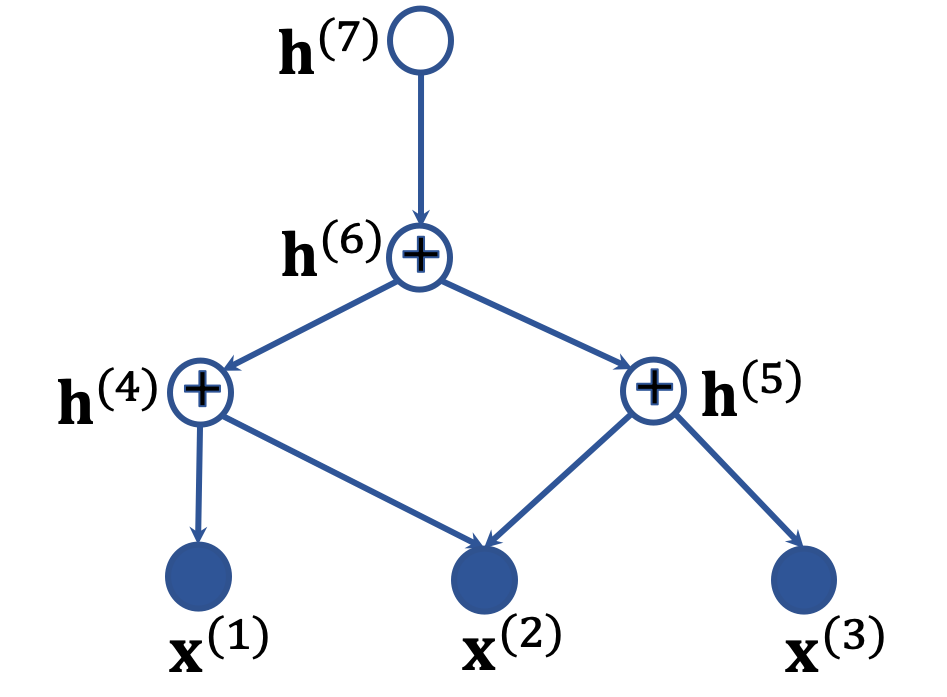
\includegraphics[width=2.3in]{fig/dag.png}
    \caption{DAG structure. The inverse topology order is \big\{ \{1,2,3\}, \{4,5\}, \{6\},  \{7\} \big\}, and it corresponds to layers 0 to 3.  }
    \label{fig:dag}
\end{figure}

By taking the topology order as the layers in tree structures, we can derive the ELBO for DAG structures.  
Assume the DAG structure has $L$ layers, and the root nodes are in layer $L$. 
We denote by $\mathbf{h}$ the vector of latent variables, then following~(\ref{eq:elbo12L}) we develop the ELBO as
\begin{align}  \label{eq:dag_elbo}
\log p(\mathbf{x})  \geqslant  \mathcal{L}(x;\theta)  = &  \mathbb{E}_{q(\mathbf{h} | \mathbf{x})} \bigg[ \log  \frac{p(\mathbf{x}, \mathbf{h})}{q(\mathbf{h}|\mathbf{x})}  \bigg]  \\ \notag
=&  \underbrace{ \mathbb{E}_{q(\mathbf{h} | \mathbf{x})} \bigg[ \log  p(\mathbf{x} |\mathbf{h})  \bigg] }_{  \parbox{10.5em}{Reconstruction of the data}}  -  \underbrace{  \mathbb{E}_{q(\mathbf{h}| \mathbf{x})} \bigg[  \log q(\mathbf{h}|\mathbf{x}) - \log p( \mathbf{h}) \bigg] }_{\textbf{\text{KL}}} \, .   \notag
\end{align} %\log  \frac{p( \mathbf{h})}{q(\mathbf{h}|\mathbf{x})} 
Similarly the KL term can be expanded as in the tree structures. 
For nodes in layer $l$
\begin{align*} 
\textbf{\text{KL}}^{l:L} 
= &\mathbb{E}_{q(\mathbf{h}^{1:L}|\mathbf{x})}\big[  \log q(\mathbf{h}^{l:L}|\mathbf{h}^{1:l-1})- \log p(\mathbf{h}^{l:L})  \big].
\end{align*} 
%\\%=&  \mathbb{E}_{q(\mathbf{h}^{1:L}|\mathbf{x})}\big[  \log q(\mathbf{h}^{l:L}|\mathbf{h}^{ch(l)})- \log p(\mathbf{h}^{l:L})  \big].
Note that $ch(l)$ may include nodes from layers lower than $l-1$, and $pa(l)$ may include nodes from layers higher than $l$.
Some nodes in $l$ may not have parent. Based on conditional independence with the topology order of a DAG, we have 
\begin{align} \label{eq:dag_chain_q}
&q(\mathbf{h}^{l:L}|\mathbf{h}^{1:l-1})=q(\mathbf{h}^{l}|\mathbf{h}^{1:l-1})q(\mathbf{h}^{l+1:L}|\mathbf{h}^{l})=q(\mathbf{h}^{l}|\mathbf{h}^{1:l-1})q(\mathbf{h}^{l+1:L}|\mathbf{h}^{1:l})\\ \label{eq:dag_chain_p}
&p(\mathbf{h}^{l:L}) =p(\mathbf{h}^{l}|\mathbf{h}^{l+1:L})p(\mathbf{h}^{l+1:L})% = p(\mathbf{h}^{l}|\mathbf{h}^{pa(l)})p(\mathbf{h}^{l+1:L}) 
\end{align}

Following~(\ref{eq:kl_lL}) and with~(\ref{eq:dag_chain_q}-\ref{eq:dag_chain_p}), we have 
 \begin{align} \notag
\textbf{\text{KL}}^{l:L} 
=&  \mathbb{E}_{q(\mathbf{h}^{1:L}|\mathbf{x})}\big[  \log q(\mathbf{h}^{l}|\mathbf{h}^{1:l-1})   - \log p(\mathbf{h}^{l}|\mathbf{h}^{l+1:L}) \big] + \underbrace{\mathbb{E}_{q(\mathbf{h}^{l:L}|\mathbf{x})}\big[  \log q(\mathbf{h}^{l+1:L}|\mathbf{h}^{1:l})- \log p(\mathbf{h}^{l+1:L})  \big]}_{\mathbf{KL}^{l+1:L}}.
\end{align}
Furthermore,
\begin{align*} 
q(\mathbf{h}^{l}|\mathbf{h}^{1:l-1})=q(\mathbf{h}^{l}|\mathbf{h}^{ch(l)}), \quad  \quad   p(\mathbf{h}^{l}|\mathbf{h}^{l+1:L}) = p(\mathbf{h}^{l}|\mathbf{h}^{pa(l)}).
\end{align*}
Hence,
 \begin{align} \label{eq:dag_kl_lL}
\textbf{\text{KL}}^{l:L} 
=&  \underbrace{\mathbb{E}_{q(\mathbf{h}^{1:L}|\mathbf{x})}\big[  q(\mathbf{h}^{l}|\mathbf{h}^{ch(l)})  - p(\mathbf{h}^{l}|\mathbf{h}^{pa(l)}) \big]}_{\textbf{\text{KL}}^{l}} +\textbf{\text{KL}}^{l+1:L} 
\end{align}
For nodes in layer $l$,
\begin{align} \notag
\textbf{\text{KL}}^{l} =& \sum_{i \in l} \underbrace{\mathbb{E}_{q(\mathbf{h}^{1:L}|\mathbf{x})}\big[  q(\mathbf{h}^{(i)}|\mathbf{h}^{ch(i)})  - p(\mathbf{h}^{(i)}|\mathbf{h}^{pa(i)}) \big]}_{\textbf{\text{KL}}^{(i)}} .
\end{align}
Recurrently applying~(\ref{eq:dag_kl_lL}) to (\ref{eq:dag_elbo}) yields
\begin{align}\notag %\label{eq:elbo_dag_1}
\mathcal{L}(\mathbf{x}; \theta) =& \mathbb{E}_{q(\mathbf{h}|\mathbf{x})}\big[ \log p(\mathbf{x}|\mathbf{h})  \big] -  \sum_{i \in \mathcal{V}  \setminus  \mathcal{R}_{ \mathcal{G} }} \textbf{\text{KL}}^{(i)} -    \sum_{i \in  \mathcal{R}_{ \mathcal{G} }  }  \textbf{\text{KL}}\big(q(\mathbf{h}^{(i)} | \mathbf{h}^{ch(i)} )   || p(\mathbf{h}^{(i)})  \big) .
\end{align}
For node $i$, 
$$\textbf{\text{KL}}^{(i)} = \mathbb{E}_{q(\mathbf{h}|\mathbf{x})}\big[  q(\mathbf{h}^{(i)}|\mathbf{h}^{ch(i)})  - p(\mathbf{h}^{(i)}|\mathbf{h}^{pa(i)}) \big].$$

\section{Model the Distributions of Latent Latent Representations at Nodes}\label{sec:vfg_inference}

Maximizing the lower bound~(\ref{eq:elbo}) equals to  optimizing the parameters of the flows, $\theta$. Different from VAEs, in a VFG all the latent variables are generated with deterministic flow functions. The calculation of the data reconstruction term in~\eqref{eq:elbo} requires  samples of both the posterior and the prior conditional distributions in each hidden layer. It corresponds to the encoding and decoding procedures in VAE model~\cite{kingma2013auto} as given by~\eqref{eq:vae_recon}. For all the layers, the samples of both posteriors and priors~are 
\begin{align} \label{eq:post_smp}
 &\mathbf{h}^l \sim q(\cdot | \mathbf{h}^{l-1})  \quad \quad \textrm{where} \quad 1\leqslant l \leqslant L \ ., \\  \label{eq:prior_smp}
 &\widehat{\mathbf{h}}^l \sim p(\cdot | \widehat{\mathbf{h}}^{l+1}) \quad \quad \textrm{where} \quad 0\leqslant l \leqslant L-1 \ .
 \end{align}
Here we use $\widehat{\mathbf{h}}^l$ to represent the sample drawn from the prior in order to discriminate it from the posterior. We also call it the reconstruction of $\mathbf{h}^l$ in the encode-decode procedures. At the root node,  we have $\widehat{\mathbf{h}}^L=\mathbf{h}^L$.  


\subsection{Distributions at Nodes}
 We assume each entry of a hidden node follows a Laplace distribution, i.e., $\mathbf{h}_j^{(i)} \sim \text{Laplace}(\mu_j^{(i)}, s_j^{(i)})$ for node $i$'s $j$th entry. Here $\mu_j^{(i)}$ is the location and $s_j^{(i)}$ is the scale. Compared to other distributions, Laplace can introduce sparsity to the model and it works well in practice. At level $l \in [L]$, we set $q(\cdot|\mathbf{h}^{l-1}) := \text{Laplace}(\mathbf{\mu}^l, \mathbf{s}^l)$ with
 
% {\color{red} s can be 1, need experiments}
 \begin{align} \notag
&\mathbf{\mu}^l = \text{median}\big(H\big), \ \  \mathbf{s}^l =\frac{1}{B}\sum_{b=1}^B|\mathbf{h}_b^l - \mathbf{\mu}^l| \ .
\end{align}
Here $H=\{\mathbf{h}^l_b| 1\leqslant b \leqslant B\}$ is a batch of latent values generated from a batch of data samples with size $B$. 
We also set the prior as $p(\cdot | \widehat{\mathbf{h}}^{l+1}):=\text{Laplace}(\widehat{\mathbf{h}}^l, 1)$. Thus for a latent variable $\mathbf{h}^l$, the log-likelihood of its construction in~(\ref{eq:kl_est}) is given by 
\begin{align} \notag
& \log p(\mathbf{h}^l | \widehat{\mathbf{h}}^{l+1}) = -\|\mathbf{h}^l- \widehat{\mathbf{h}}^l\|_1 -d\cdot\log2  .
\end{align}
Here $d = dim(\mathbf{h}^l)$. Hence, minimizing  $\mathbf{KL}$s is to minimize the $\ell_1$ distance between latent variables and their reconstructions. In practice, we set $M=1$ for efficiency. With a batch of training samples, $\mathbf{x}_b, 1 \leqslant b \leqslant B$, the structure of flow functions make the  forward  and  backward message passing very efficient, and  thus the estimation of the ELBO.  

If several nodes have multiple parents, the graph will be a DAG. It is easy to extend the computation of the ELBO~(\ref{eq:elbo}) to DAGs with topology ordering of the nodes (and thus of the layers). 
Let $ch(i)$ and $pa(i)$ denote node $i$'s child set and parent set, respectively.
Then, the ELBO for a DAG structure reads:
\begin{align}\label{eq:elbo_dag}
\mathcal{L}(\mathbf{x}; \theta) =& \mathbb{E}_{q(\mathbf{h}|\mathbf{x})}\big[ \log p(\mathbf{x}|\mathbf{h})  \big] -  \sum_{i \in \mathcal{V}  \setminus  \mathcal{R}_{ \mathcal{G} }} \textbf{\text{KL}}^{(i)}   -    \sum_{i \in  \mathcal{R}_{ \mathcal{G} }  }  \textbf{\text{KL}}\big(q(\mathbf{h}^{(i)} | \mathbf{h}^{ch(i)} )   || p(\mathbf{h}^{(i)})  \big) .
\end{align}
Here $\mathbf{KL}^{(i)}=\mathbb{E}_{q(\mathbf{h}|\mathbf{x})}\big[  \log q(\mathbf{h}^{(i)}|\mathbf{h}^{ch(i)})   - \log p(\mathbf{h}^{(i)}|\mathbf{h}^{pa(i)}) \big]$. $\mathcal{V}$ stands for the node set of DAG $\mathcal{G} = \{\mathcal{V}, \mathbf{f}\}$, and $\mathcal{R}_{ \mathcal{G}}$ is the set of root or source nodes. 
 
Assuming there are $k$ leaf nodes on a tree or a DAG model, corresponding to $k$ sections of the input sample $\mathbf{x} = [\mathbf{x}^{(1)}, ..., \mathbf{x}^{(k)}]$, then the hidden variables in both~(\ref{eq:elbo}) and~(\ref{eq:elbo_dag}) are computed with forward and backward message passing. 
Next, we provide more details about the nodes.


\vspace{-0.1in}
\subsubsection{KL Computation for Nodes}
The expectation of the reconstruction term in ELBO~(\ref{eq:elbo}) can be approximated with $M$ samples, 
\begin{align*} 
&\mathbb{E}_{q(\mathbf{h}^{1:L}|\mathbf{x})}\big[ \log p(\mathbf{x}|\mathbf{h}^{1:L})\big]
=\mathbb{E}_{q(\mathbf{h}^{1:L}|\mathbf{x})}\big[ \log p(\mathbf{x}|\widehat{\mathbf{h}}^{1:L})  \big] \\
&\simeq \frac{1}{M}\sum_{m=1}^M \log p(\mathbf{x}| \widehat{\mathbf{h}}^{1:L}_m) = \frac{1}{M}\sum_{m=1}^M \log p(\mathbf{x}| \widehat{\mathbf{h}}^{1}_m) .
 \end{align*}
 Here $\widehat{\mathbf{h}}^{1:L}_m$ is the $m$th draw of the prior distribution with  $\widehat{\mathbf{h}}^{l}_m$ sampled according to~(\ref{eq:prior_smp}), and the root latent variable sampled from the posterior, i.e. $\widehat{\mathbf{h}}^{L}_m=\mathbf{h}^{L}_m \sim q(\cdot | \mathbf{h}^{L-1}) $. The computation of $ \mathbf{h}^l$s and $\widehat{\mathbf{h}}^l$s with~(\ref{eq:post_smp}) and~(\ref{eq:prior_smp}) are considered as the forward and backward message passing, respectively~(shown in Figure~\ref{fig:message}). They also are considered as encoding and decoding procedures in the auto-encoder manner~\cite{kingma2013auto}. 
 
\begin{figure}[H]
\begin{center}
 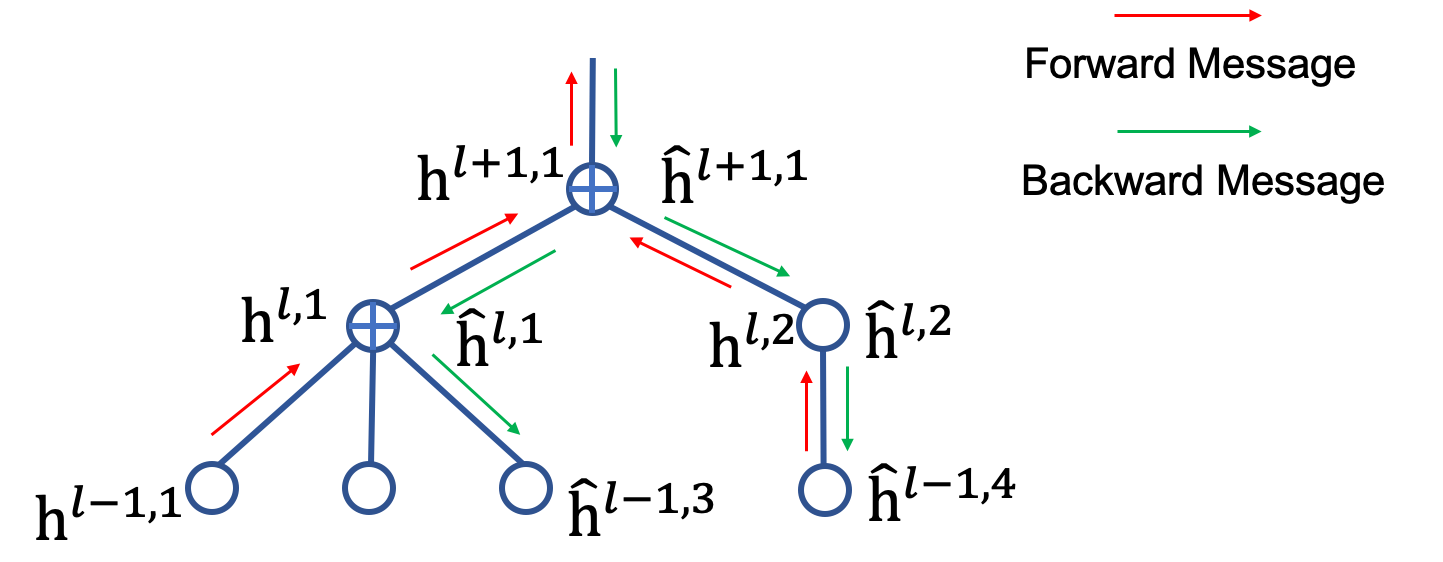
\includegraphics[width=0.6\linewidth]{fig/message.png}
\end{center}
\vspace{-0.2in}
\caption{ {\small  Layer-wise sampling of the posterior and the prior corresponds to forward~(encoding) and backward~(decoding) message passing, respectively.}}
\label{fig:message}
\vspace{-0.15in}
\end{figure}

For any $l \in [L]$, the calculation of the $\mathbf{KL}^l$ term is done in a similar manner, and \eqref{eq:kl} can be approximated with 
\begin{align*}
\mathbf{KL}^l&=\mathbb{E}_{q(\mathbf{h}^{1:L}|\mathbf{x})}\big[  \log q(\mathbf{h}^{l}|\mathbf{h}^{l-1})   - \log p(\mathbf{h}^{l}|\widehat{\mathbf{h}}^{l+1}) \big] \simeq \frac{1}{M}\sum_{m=1}^M\big[ \log q(\mathbf{h}_m^{l}|\mathbf{h}^{l-1})   - \log p(\mathbf{h}_m^{l}|\widehat{\mathbf{h}}_m^{l+1})  \big].
\end{align*}
The $m$th sample is generated with~(\ref{eq:post_smp}), and $\widehat{\mathbf{h}}_m^{l+1}$ with~(\ref{eq:prior_smp}).  

Adjacent layers are connected with one or multiple flow functions, and the prior and posterior use the same structure.  We follow the approach in~\cite{rezende2015variational,berg2018sylvester}  using normalizing flows to improve ELBO estimation. The $\mathbf{KL}$ term can be improved as
\begin{align} \label{eq:kl_est}
\mathbf{KL}^l
\simeq & \frac{1}{M}\sum_{m=1}^M\bigg[ \log q(\mathbf{h}^{l}_m|\mathbf{h}^{l-1}) +\log \bigg|\det \frac{\partial \mathbf{h}^{l}_m}{\partial \mathbf{h}^{l+1}_m}\bigg| + \log \bigg|\det \frac{\partial \widehat{\mathbf{h}}^{l+1}_m}{\partial \widehat{\mathbf{h}}^{l}_m}\bigg|   - \log p(\mathbf{h}^{l}_m|\widehat{\mathbf{h}}_m^{l+1}) \bigg].
\end{align}

\section{More Details on Inference}
%We present in this section the proofs for our Lemma~\ref{lm:apprx} and Theorem~\ref{thm:identif}.
\subsection{Inference on DAGs}

\begin{figure}[H]
\begin{center}
 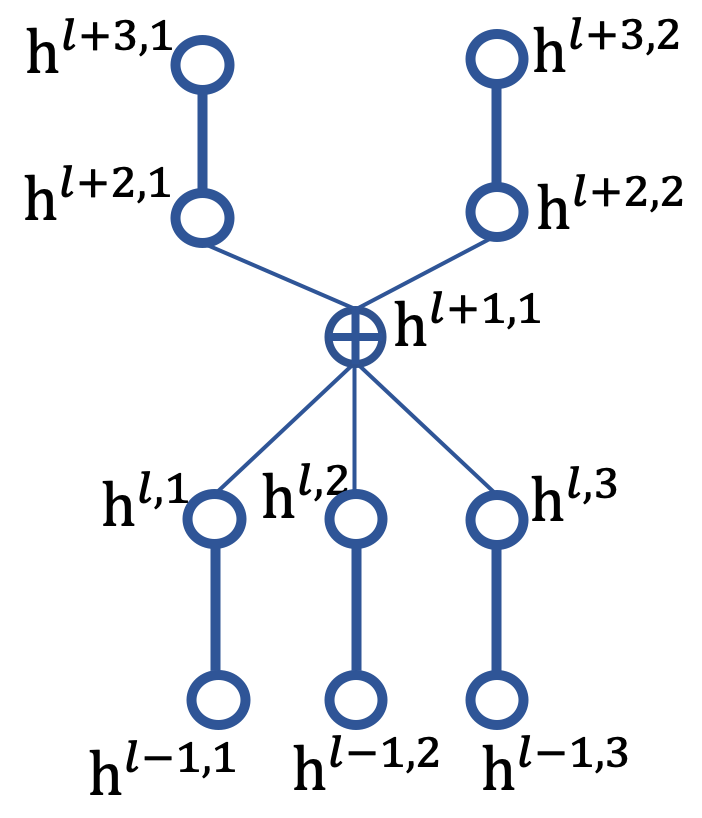
\includegraphics[width=0.25\linewidth]{fig/dag_aggr.png}
\end{center}
\vspace{-0.2in}
\caption{ {\small  Aggregation node in a DAG.}}
\label{fig:dag_aggr}
\vspace{-0.15in}
\end{figure}

% \subsection{ Inference Reliability and  Expressive Power}
% \subsubsection{Prediction Error }




\subsection{Proof of Lemma~\ref{lm:apprx}}\label{appd:proof_lm1}
\textbf{Lemma 1.} {\it Let $\mathcal{G}$ be a well trained tree structured variational flow graphical model with $L$ layers, and $i$ and $j$ are two leaf nodes with $a$ as the closest common ancestor. 
Given observed value at node $i$, the value of node $j$ can be approximated with $\widehat{\mathbf{x}}^{(j)} \approx  \mathbf{f}_{(a,j)}(\mathbf{f}_{(i, a)}(\mathbf{x}^{(i)}))$. Here $\mathbf{f}_{(i, a)}$ is the flow function path from node $i$ to node $a$. 
The conditional density of $\mathbf{x}^{(j)}$ given $\mathbf{x}^{(i)}$ can be approximated with 
\begin{align*} %\label{eq:cond_llk}
\log p(\mathbf{x}^{(j)} | \mathbf{x}^{(i)}) &\approx  \log p(\widehat{\mathbf{h}}^L) -  \frac{1}{2} \log \big(\det \big(\mathbf{J}_{\widehat{\mathbf{x}}^{(j)}}(\widehat{\mathbf{h}}^L)^\top\mathbf{J}_{\widehat{\mathbf{x}}^{(j)}}(\widehat{\mathbf{h}}^L)\big) \big) \, .
\end{align*}
}

\begin{proof}
Without loss generality, we assume that there are relationships among different data sections, and the value of one section can be partially or approximately imputed by other sections. 
According to the aggregation rule (b) discussed in section~\ref{sec:node_aggr}, at an aggregation node  $a$, the latent value of a child node $j$ has the same reconstruction value as the parent node.  
The reconstruction of the child node $j$ can be approximated with the reconstruction of the parent node, i.e., $\widehat{\mathbf{h}}^{(j)} \approx \mathbf{f}_{(a,j)}(\widehat{\mathbf{h}}^{a)})$. 
Recalling the reconstruction term in the ELBO~(\ref{eq:elbo}), at each node we have $\mathbf{h}^{(a)} \approx \widehat{\mathbf{h}}^{(a)}$. Hence for node $a$'s descendent $j$, we have $\widehat{\mathbf{h}}^{(j)} \approx \mathbf{f}_{(a,j)}(\mathbf{h}^{(a)})$, and $\mathbf{f}_{(a,j)}$ is the flow function path from $a$ to $j$. 
The value of node $a$ can be approximated by the value of its descendent $i$ that has observation, i.e., $\mathbf{h}^{(a)} \approx \mathbf{f}_{(i,a)}(\mathbf{h}^{(i)})$. Hence, we have $\widehat{\mathbf{x}}^{(j)} \approx  \mathbf{f}_{(a,j)}(\mathbf{f}_{(i, a)}(\mathbf{x}^{(i)}))$.

To compute  node $j$'s conditional distribution given the observed node $i$, we can use the forward passing to compute the root's reconstruction  value $\widehat{\mathbf{h}}^L$. 
Node $j$'s reconstruction value $\widehat{\mathbf{x}}^{(j)}$ can be imputed by backward passing the message at the root. The density value of $\widehat{\mathbf{h}}^L$ can be computed with the prior distribution of the root. The conditional density of $\widehat{\mathbf{x}}^{(j)}$ can be computed using the change of variable theorem, and it is known in the context of geometric measure theory ~\cite{Book:Hanson_1994,Article:Krantz_2008}. It reads 
\begin{align*} %\label{eq:llk_est1}
&  p(\mathbf{x}^{(j)} | \mathbf{x}^{(i)} ) \approx p(\widehat{\mathbf{h}}^L)\det\big(\mathbf{J}_{\widehat{\mathbf{x}}^{(j)}}(\widehat{\mathbf{h}}^L)^\top  \mathbf{J}_{\widehat{\mathbf{x}}^{(j)}}(\widehat{\mathbf{h}}^L\big)^{-\frac{1}{2}}.
\end{align*}
Applying the logarithm operator on both sides concludes the proof of our Lemma.
\end{proof}


\subsection{ Inference Reliability and  Expressive Power}


\subsubsection{Prediction Error }

\begin{theorem}
Algorithm 2 can ensure the aggregation nodes capture the relations. Optimizing the objective ensure parents and child share similar value, i.e., 
\end{theorem}

\begin{proof}

$\mathbf{KL}^{(i)}=\mathbb{E}_{q(\mathbf{h}|\mathbf{x})}\big[  \log q(\mathbf{h}^{(i)}|\mathbf{h}^{ch(i)})   - \log p(\mathbf{h}^{(i)}|\mathbf{h}^{pa(i)}) \big]$
\begin{align} \notag
& \log p(\mathbf{h}^l | \widehat{\mathbf{h}}^{l+1}) = -\|\mathbf{h}^l- \widehat{\mathbf{h}}^l\|_1 -d\cdot\log2  .
\end{align}

\end{proof}

%Average aggregation.

%{\color{red} Neural network learning theory; approximation theory}

%DAG


\subsubsection{ Probability Tractability}
%{\color{red} Neural Graphical model theory! }
\begin{theorem}
With Algorithm 2,  we can compute the marginal and conditional probability of nodes. 
\end{theorem}





\section{Theoretical Justifications for Latent Representation Learning}\label{sec:theory}

The proposed Variational Flow Graphical models provide approaches to integrate multi-modal (multiple natures of data) or multi-source (collected from various sources) data. 
With invertible flow functions, we analyze the identifiability~\cite{Khemakhem20a,Sorrenson2020} of the VFG in this section.  
We assume that each input data point has $k$ sections, and denote by $\mathbf{h}^{(t)}$, the latent variable for section $t$, namely $\mathbf{x}^{(t)}$. 
Suppose the distribution of the latent variable $\mathbf{h}^{(t)}$, conditioned on $\mathbf{u}$, is a factorial member of the exponential family with $m > 0$ sufficient statistics, see \cite{efron1975defining} for more details on exponential families. 
Here $\mathbf{u}$ is an additional observed variable which can be considered as covariates.
The general form of the exponential distribution can be expressed as 
\begin{equation}\label{eq:exp_h}
\begin{split}
&p_{\mathbf{h}^{(t)}}(\mathbf{h}^{(t)} | \mathbf{u})  = \Pi_{i=1}^d \frac{Q_i(h^{(t,i)})}{Z_i(\mathbf{u})} \text{exp}\bigg[ \sum_{j=1}^m T_{i,j}(h^{(t,i)}) \lambda_{i,j}(\mathbf{u}) \bigg]\, ,
\end{split}
\end{equation} 
where $Q_i$ is the base measure, $Z_i(\mathbf{u})$ is the normalizing constant, $T_{i,j}$ are the component of the sufficient statistic and $\lambda_{i,j}$ the corresponding parameters, depending on the variable $\mathbf{u}$. 
Data section variable $\mathbf{x}^{(t)}$ is generated with some complex, invertible, and deterministic function from the latent space as in: 
\begin{align}\label{eq:xt_gen}
\mathbf{x}^{(t)} = \mathbf{f}^{-1}_t(\mathbf{h}^{(t)}, \epsilon)\, ,
\end{align}
%Shaogang: here \epsilon should be stated in this way, no more changes!
where $\epsilon$ is some additional random noise in the generation of $\mathbf{x}^{(t)}$. 
Let $\mathbf{T} =[\mathbf{T}_1, ..., \mathbf{T}_d] $, and $\mathbf{\lambda} =[\mathbf{\lambda}_1, ..., \mathbf{\lambda}_d]$.  
 We define the domain of the inverse flow $\mathbf{f}_t^{-1}$ as $\mathcal{H}=\mathcal{H}_1 \times ... \times \mathcal{H}_d$.
The parameter set $\widehat{\Theta} = \{\widehat{\mathbf{\theta}} := (\widehat{\mathbf{T}}, \widehat{\mathbf{\lambda}}, \mathbf{g} ) \}$ is defined in order to represent the model learned by a piratical algorithm. Let $\mathbf{z}^{(t)}$ be one sample's latent variable recovered by the algorithm regarding $\mathbf{h}^{(t)}$.
In the limit of infinite data and algorithm convergence, we establish the following theoretical result regarding the identifiability of the sufficient statistics $\mathbf{T}$ in our model~(\ref{eq:exp_h}).


% The proof of Theorem~\ref{thm:identif} and further analysis can be found in the supplementary file. 

\textbf{Theorem 1.} {\it 
Assume that the observed data is distributed according to the model given by~(\ref{eq:exp_h}) and~(\ref{eq:xt_gen}).
Let the following assumptions holds,

\vspace{0.05in}
(a) The sufficient statistics $T_{ij}(h)$ are differentiable almost everywhere and their derivatives $ \partial T_{i,j}/\partial_h$ are nonzero almost surely for all $h\in \mathcal{H}_i$, $1\leqslant i \leqslant d$ and $1 \leqslant j  \leqslant m$.

\vspace{0.05in}
(b) There exist $(dm+1)$ distinct conditions $\mathbf{u}^{(0)}$, ..., $\mathbf{u}^{(dm)}$  such that the matrix 
\begin{equation*} 
\mathbf{L} = [\mathbf{\lambda}(\mathbf{u}^{(1)}) - \mathbf{\lambda}(\mathbf{u}^{(0)}), ..., \mathbf{\lambda}(\mathbf{u}^{(dm)}) - \mathbf{\lambda}(\mathbf{u}^{(0)}) ]
\end{equation*} 
of size $dm \times dm$ is invertible.

Then the model parameters 
$\mathbf{T}(\mathbf{h}^{(t)}) = \mathbf{A}\widehat{\mathbf{T}}(\mathbf{z}^{(t)}) + \mathbf{c}.$ Here $\mathbf{A}$ is a $dm \times dm$ invertible matrix and $\mathbf{c}$ is a vector of size $dm$.
}

\begin{proof}
The conditional probabilities of $p_{\mathbf{T}, \mathbf{\lambda}, \mathbf{f}_t^{-1} }\big(\mathbf{x}^{(t)} | \mathbf{u}\big)$ and $p_{\widehat{\mathbf{T}}, \widehat{\mathbf{\lambda}}, \mathbf{g} }\big(\mathbf{x}^{(t)} | \mathbf{u}\big)$ are assumed to be the same in the limit of infinite data.  
By expanding the probability density functions with the correct change of variable, we have 
\begin{align} \notag
\log p_{\mathbf{T}, \mathbf{\lambda}}(\mathbf{h}^{(t)}| \mathbf{u}) + \log \big| \det \mathbf{J}_{\mathbf{f}_t}(\mathbf{x}^{(t)}) \big| = \log p_{\widehat{\mathbf{T}}, \widehat{\mathbf{\lambda}}}(\mathbf{z}^{(t)}| \mathbf{u}) + \log \big| \det \mathbf{J}_{g^{-1}}(\mathbf{x}^{(t)}) \big|.
\end{align}
Let $\mathbf{u}^{(0)},...,\mathbf{u}^{(dm)}$ be from condition (b). We can subtract this expression of $\mathbf{u}^{(0)}$ from some  $\mathbf{u}^{(v)}$. The Jacobian terms will be removed since they do not depend  $\mathbf{u}$,
\begin{align} \label{eq:u_diff}
\log p_{\mathbf{h}^{(t)}}(\mathbf{h}^{(t)}|\mathbf{u}^{(v)}) - \log p_{\mathbf{h}^{(t)}}(\mathbf{h}^{(t)}|\mathbf{u}^{(0)}) =\log p_{\mathbf{z}^{(t)}}(\mathbf{z}^{(t)}|\mathbf{u}^{(v)}) - \log p_{\mathbf{z}^{(t)}}(\mathbf{z}^{(t)}|\mathbf{u}^{(0)}) .
\end{align}
Both conditional distributions in~\eqref{eq:u_diff} belong to the exponential family. 
Eq.~(\ref{eq:u_diff}) thus reads
\begin{align} \notag
&\sum_{i=1}^d \bigg[\log \frac{Z_i(\mathbf{u}^{(0)})}{Z_i(\mathbf{u}^{(v)})} + \sum_{j=1}^m T_{i,j}(\mathbf{h}^{(t)})\big(\lambda_{i,j}(\mathbf{u}^{(v)})- \lambda_{i,j}(\mathbf{u}^{(0)})\big) \bigg] \\ \notag
= & \sum_{i=1}^d \bigg[\log \frac{\widehat{Z}_i(\mathbf{u}^{(0)})}{\widehat{Z}_i(\mathbf{u}^{(v)})} + \sum_{j=1}^m \widehat{T}_{i,j}(\mathbf{z}^{(t)})\big(\widehat{\lambda}_{i,j}(\mathbf{u}^{(v)})- \widehat{\lambda}_{i,j}(\mathbf{u}^{(0)})\big) \bigg].
\end{align}
Here the base measures $Q_i$s are canceled out. 
Let $\bar{\mathbf{\lambda}}(\mathbf{u}) = \mathbf{\lambda}(\mathbf{u})-\mathbf{\lambda}(\mathbf{u}^{(0)})$. 
The above equation can be expressed, with inner products, as follows
\begin{align} \notag
\langle \mathbf{T}(\mathbf{h}^{(t)}), \bar{\mathbf{\lambda}}	\rangle + \sum_i \log \frac{Z_i(\mathbf{u}^{(0)})}{Z_i(\mathbf{u}^{(v)})}
=\langle \widehat{\mathbf{T}}(\mathbf{z}^{(t)}), \bar{\widehat{\mathbf{\lambda}}}	\rangle + \sum_i\log \frac{\widehat{Z}_i(\mathbf{u}^{(0)})}{\widehat{Z}_i(\mathbf{u}^{(v)})}, \ \ \forall \ v, 1 \leqslant v \leqslant dm .
\end{align}
Combine $dm$ equations together and we can rewrite them in matrix equation form as following
\begin{align} \notag
\mathbf{L}^{\top}\mathbf{T}(\mathbf{h}^{(t)}) = \widehat{\mathbf{L}}^{\top}\widehat{\mathbf{T}}(\mathbf{z}^{(t)}) + \mathbf{b}.
\end{align}
Here $b_v=\sum_{i=1}^{d}\log \frac{\widehat{Z}_i(\mathbf{u}^{(0)}) Z_i(\mathbf{u}^{(v)}) }{\widehat{Z}_i(\mathbf{u}^{(v)}) Z_i(\mathbf{u}^{(0)}) }$. We can multiply $\mathbf{L}^{\top}$'s inverse with both sized of the equation, 
\begin{align}\label{eq:A_sim}
\mathbf{T}(\mathbf{h}^{(t)}) = \mathbf{A}\widehat{\mathbf{T}}(\mathbf{z}^{(t)}) + \mathbf{c}.
\end{align}
Here $\mathbf{A} = \mathbf{L}^{-1\top} \widehat{\mathbf{L}}^{\top} $, and $\mathbf{c} = \mathbf{L}^{-1\top} \mathbf{b}$. 
By Lemma 1 from~\cite{Khemakhem20a}, there exist $m$ distinct values $h^{(t),i}_{1}$ to $h^{(t),i}_{m}$ such that $\big[ \frac{d T_i}{ d h^{(t),i}}(h^{(t),i}_{1}), ...,  \frac{d T_i}{ d h^{(t),i}}(h^{(t),i}_{m}) \big]$ are linearly independent in $\mathbb{R}^m$, for all $1\leqslant i \leqslant d$. 
Define $m$ vectors $\mathbf{h}^{(t)}_{v}= [h^{(t),1}_v, ..., h^{(t),d}_v]$ from points given by this lemma. 
We obtain the following Jacobian matrix
$$\mathbf{Q}= [\mathbf{J}_{\mathbf{T}}(\mathbf{h}^{(t)}_1), ..., \mathbf{J}_{\mathbf{T}}(\mathbf{h}^{(t)}_m)] \, ,$$ 
where each entry is the Jacobian of size $dm \times d$ from the derivative of Eq.~(\ref{eq:A_sim}) regarding the $m$ vectors $\{\mathbf{h}^{(t)}_j\}_{j=1}^m$. 
Hence $\mathbf{Q}$ is a $dm \times dm$ invertible by the lemma and the fact that each component of $\mathbf{T}$ is univariate. %% m =k, d=n, v = l. i index for d
We can construct a corresponding matrix $\widehat{\mathbf{Q}}$ with the Jacobian of $\widehat{\mathbf{T}}(\mathbf{g}^{-1}\circ \mathbf{f}_t^{-1}(\mathbf{h}^{(t)}))$ computed at the same points and get 
\begin{align} \notag
\mathbf{Q} = \mathbf{A}\widehat{\mathbf{Q}} \,.
\end{align}
Here $\widehat{\mathbf{Q}}$ and $\mathbf{A}$ are both full rank as $\mathbf{Q}$ is full rank.
\end{proof}

According to Theorem 1, the proposed model not only can identify global latent factors, but also identify the latent factors for each section with enough auxiliary information. 
VFG provides a potential approach to learn the latent hierarchical structures from datasets.



\end{document}
